% !TeX TXS-program:compile = txs:///arara
% arara: pdflatex: {shell: yes, synctex: no, interaction: batchmode}
% arara: pdflatex: {shell: yes, synctex: no, interaction: batchmode} if found('log', '(undefined references|Please rerun|Rerun to get)')

\documentclass[french,11pt,a4paper]{article}
\usepackage[utf8]{inputenc}
\usepackage[T1]{fontenc}
\RequirePackage[upright]{fourier}
\RequirePackage{mathtools}
\RequirePackage{amsmath,amssymb,amstext}
\RequirePackage[scaled=0.875]{helvet}
\renewcommand\ttdefault{lmtt}
\RequirePackage[scaled=0.925]{cabin} % sf
%\usepackage{DejaVuSerif}
%\usepackage[scale=1.1]{inconsolata}
\usepackage[pastableur]{customenvs}
\usepackage{tabularx}
\usepackage{soul}
%\usepackage{codehigh}
%\usepackage{fontawesome5}
\usepackage{lipsum}
\usepackage{fancyvrb}
\usepackage{fancyhdr}
\fancyhf{}
\renewcommand{\headrulewidth}{0pt}
\lfoot{\sffamily\small [customenvs]}
\cfoot{\sffamily\small - \thepage{} -}
\rfoot{\hyperlink{matoc}{\small\faArrowAltCircleUp[regular]}}
\usepackage{hologo}
\providecommand\tikzlogo{Ti\textit{k}Z}
\providecommand\TeXLive{\TeX{}Live\xspace}
\providecommand\PSTricks{\textsf{PSTricks}\xspace}
\let\pstricks\PSTricks
\let\TikZ\tikzlogo

\usepackage{hyperref}
\urlstyle{same}
\hypersetup{pdfborder=0 0 0}
\usepackage[margin=1.5cm]{geometry}
\setlength{\parindent}{0pt}

\def\TPversion{0.40c}
\def\TPdate{23 juin 2025}
\usepackage{tcolorbox}
\tcbuselibrary{listingsutf8}
%\usepackage{eurosym}
\newtcblisting{DemoCode}[1]{%
	enhanced,width=0.95\linewidth,center,%
	bicolor,size=title,%
	colback=cyan!5!white,%
	colbacklower=cyan!1!white,%
	colframe=cyan!75!black,%
	listing options={%
		inputencoding=utf8,
		%literate={`E}{{€}}{1},
		breaklines=true,%
		breakatwhitespace=true,%
		style=tcblatex,basicstyle=\small\ttfamily,%
		tabsize=4,%
		commentstyle={\itshape\color{gray}},
		keywordstyle={\color{blue}},%
		classoffset=0,%
		keywords={usepackage,displaystyle,frac,infty,begin,end,lipsum,centering,par,baselineskip,item,bullet,int,color,NewDocumentCommand},%
		alsoletter={-},%
		keywordstyle={\color{blue}},%
		classoffset=1,%
		alsoletter={-},%
		morekeywords={center,justify,\LstDeuxNiv,\LstTroisNiv,\LstQuatreNiv,\NoticeDeuxNiv,\NoticeTroisNiv,\NoticeQuatreNiv,\DeuxNivBatterie,\TroisNivBatterie,\QuatreNivBatterie,\DeuxNivSmiley,\TroisNivSmiley,\QuatreNivSmiley,\vcenterfa,\faIcon,part,RenewDocumentCommand,IfBooleanTF},%
		keywordstyle={\color{violet}},%
		classoffset=2,%
		alsoletter={-},%
		morekeywords={\ReponsesQCM,MultiCols,\CreerListeItems,\ListeChoixItems,\TableauCompetences,\CrayonDeCompetences,\StyleEnvtExo,\StyleEnvtExoDefaut,\TitreExo,\ipsum,EnvSMS,\SMSrec,\SMSenv,BoiteSimple,\SujetTitreExo,\CircledNumber,\AffVignette,\BoiteArrondie,\ChangerDisplaySkip,\celcouleur,\celfusion,\lignetxt,\colonnetxt,\celnumbreak,\celtxt,\BandeauScore,\InsererImage,\tkzBannerTri,\tkzBannerTriAlt,\NiveauDiffExos,\tkzEtoiles,\tkzGrilleAuto,\tkzAutoGridLocal,\tkzAutoGridActivate,\tkzFlecheEvasee,PanneauAutoroute,\AfficheSoldes,\tbcmarker,\VilleDist,\RoueNiveaux,EnvRoueNiveaux,\PlacerIconeNiveau,\PlacerIconesNiveaux,\MiniCompteurNiveaux,\tkzspeedometer,AnnoterImage,\PlacerTxtSurImg,\pictoskills,\pictoskillsgreen,\pictoskillsorange,\pictoskillsred,\pictobullseye,\tkzpicto,\pictotraffic,\pictocalendar,\getwideststring,\halignmakebox,\storewidthtolength,\storeheighttolength,\storetotalheighttolength,\storedepthtolength},%
		keywordstyle={\color{green!50!black}},%
		classoffset=3,%
		morekeywords={Largeur,Filets,EspacesCL,NbCols,Labels,Melange,PoliceLabels,EspaceLabels,Swap,Type,CoeffEspVert,EpTrait,Alea,LargeurNivs,Niveaux,NoticeNiveaux,Titre,PolTitre,PolNotice,PolComp,LigneSep,CouleurNotice,CouleurNiveaux,CouleurFond,Note,Notice,PoliceCateg,PoliceBloc,Couleurs,LargeurBloc,Echelle,NoirBlanc,Libelle,EpTrait,Police,Type,ComplementTitre,Titre,CodeDebut,Couleur,EchelleImage,Decoration,Trait,Avatar,AffAvatar,NoirBlanc,CouleurE,CouleurR,CouleurFond,Hauteur,Largeur,PoliceTxt,CouleurTitre,AlignH,bg,txt,bthick,bcol,raise,Type,EspH,Fond,Texte,Style,Dense,Avant,AvantS,Apres,ApresS,Global,align,width,Legende,CouleurFond,Hauteur,Ratio,AffLegende,Couleurs,EchelleSymboles,Symboles,vRemplir,vOffset,vCentrer,height,width,blockwidth,collight,colmedium,coldar,coltxt,fonttxt,swap,maincolor,logo,type,num,dispblock,customtype,Couleur,AlignV,Offset,NiveauMax,pasX,pasY,grilleauto,TailleFleche,Direction,Coeff,TypeFleche,Deplacement,LineCap,Epaisseur,CouleurCartouche,Fleches,CouleurFond,CouleurTitre,PoliceCartouche,TypeFleche,EspacementV,OffsetFleches,Dernier,PoliceEntete,PolicePrix,PoliceReduc,OffsetReduc,AgrandirReduc,Rayon,Police,ListeNiveaux,Marqueur,Pos,Echelle,Couleurs,Taille,custommulti,Noeud,Grille,SousGrille,CouleurGrille,Clip,col,hoffset,maincolor,height,colors,listcolors},%
		keywordstyle={\color{orange}}
	},%
	#1
}
\sethlcolor{lightgray!25}
\NewDocumentCommand\MontreCode{ m }{%
	\hl{\vphantom{\texttt{pf}}\texttt{#1}}%
}
\usepackage[auto,outline]{contour}

\usepackage{babel}

\begin{document}

\pagestyle{fancy}

\thispagestyle{empty}

\begin{center}
	\begin{minipage}{0.75\linewidth}
	\begin{tcolorbox}[colframe=yellow,colback=yellow!15]
		\begin{center}
			\renewcommand\arraystretch{1.25}
			\begin{tabular}{c}
				{\Huge \texttt{customenvs [fr]}}\\
				\\
				{\Large Quelques environnements classiques,} \\
				{\Large légèrement modifiés, et basés} \\
				{\Large sur des environnements existants.} \\
			\end{tabular}
			\renewcommand\arraystretch{1}
			
			\medskip
			
			{\small \texttt{Version \TPversion{} -- \TPdate}}
		\end{center}
	\end{tcolorbox}
\end{minipage}
\end{center}

\vspace*{1mm}

\begin{center}
	\begin{tabular}{c}
	\texttt{Cédric Pierquet}\\
	{\ttfamily c pierquet -- at -- outlook . fr}\\
	\texttt{\url{https://forge.apps.education.fr/pierquetcedric/packages-latex}}
\end{tabular}
\end{center}

\vspace*{5mm}

%\hrule
%
%\vspace*{2mm}
%
%{\centering Le nom du package vient de \textsf{ENVironnemenTS ALTernatifs}, avec le suffixe \textsf{FRançais}.\par}
%
%\vspace*{2mm}
%
%\hrule
%
%\vspace*{1cm}

\hrule

\phantomsection

\hypertarget{matoc}{}

\tableofcontents

\vspace*{5mm}

\hrule

\pagebreak

\section{Historique}

\verb|v0.40c|~:~~~PictoClippy (\textsf{customenvs-tikzpictos} \texttt{v0.1.3}) + Gestion de longueurs

\verb|v0.40b|~:~~~PictoCalendar (\textsf{customenvs-tikzpictos} \texttt{v0.1.2}) + Améliorations

\verb|v0.40a|~:~~~PictoTraffic (\textsf{customenvs-tikzpictos} \texttt{v0.1.1}) + Améliorations

\verb|v0.3.7|~:~~~Externalisation des pictogrammes dans un package auxiliaire, \textsf{customenvs-tikzpictos}

\verb|v0.3.6|~:~~~Ajout d'un pictogramme \textsf{cible/flèche}

\verb|v0.3.5|~:~~~Bugfix + pre-compatibilité \textsf{fa5/6}

\verb|v0.3.4|~:~~~Pictoskill + option pour le package \textsf{adjustbox}

\verb|v0.3.3|~:~~~Annoter une image

\verb|v0.3.2|~:~~~Version alternative de la bannière \textsf{Tri}

\verb|v0.3.1|~:~~~Ajout des cases à cocher pour les \textsf{QCM}

\verb|v0.3.0|~:~~~Compatibilité accrue avec \textsf{beamer}

\verb|v0.2.7|~:~~~Clé \texttt{[Melange]} pour les QCMs

\verb|v0.2.6|~:~~~Roue des compétences / speedometer

\verb|v0.2.5|~:~~~Correction du fonctionnement de \texttt{EnvtExo}

\verb|v0.2.4|~:~~~Petite boîte type \textit{marker}

\verb|v0.2.3|~:~~~Panneaux autoroutiers + Affichettes de soldes

\verb|v0.2.2|~:~~~Ajout d'une commande pour des flèches évasées, en \TikZ\

\verb|v0.2.1|~:~~~Amélioration de la gestion des étoiles pour des niveaux de difficultés + Grille auto pour \TikZ\

\verb|v0.2.0|~:~~~Étoiles pour des niveaux de difficultés (compatible avec \texttt{EnvtExo})

\verb|v0.1.9|~:~~~Bannière de titre + Insertion d'images en remplissage vertical

\verb|v0.1.8|~:~~~Nutriscore

\verb|v0.1.7|~:~~~Possibilité de créer des vignettes \textsf{perso}

\verb|v0.1.6|~:~~~Patch \textsf{displayskip} + Patches \textsf{pas-tableur}

\verb|v0.1.5|~:~~~La librairie \texttt{babel} de \TikZ\ n'est plus chargée

\verb|v0.1.5|~:~~~Vignettes + Numéros encerclés + Création de boîtes 'simples'

\verb|v0.1.4|~:~~~Commande pour du texte dans une boîte arrondie, de hauteur 'figée' + 'Chat' SMS

\verb|v0.1.3|~:~~~Environnement/commande pour des exercices, avec personnalisation(s)

\verb|v0.1.2|~:~~~Crayon de compétences

\verb|v0.1.1|~:~~~Tableaux de compétences

\verb|v0.1.0|~:~~~Version initiale

\pagebreak

\section{Le package customenvs}

\subsection{Idée}

L'idée est de proposer des commandes ou environnements classiques avec quelques éléments de personnalisation (via des \textsf{clés} francisées), comme :

\begin{itemize}
	%\item modifier localement l'\textit{alignement vertical} d'éléments sans jambage ;
	\item \textit{centrer} avec gestion des espacements autour ;
	\item écrire en \textit{multi-colonnes} avec gestion des espacements autour ;
	\item mettre en forme des réponses à des \textit{QCM} ;
	\item créer une liste avec \textit{choix des items} (de manière aléatoire ou par saisie directe) ;
	\item créer un tableau de \textit{compétences}.
\end{itemize}

\smallskip

L'idée globale est de proposer des environnements clé en main, avec personnalisations \textit{explicites}, sans forcément avoir besoin de \textit{se pencher sur le code}, mais il est évident qu'il existe d'autres solutions pour l'utilisateur qui souhaite réellement contrôler son rendu.

\smallskip

Il est ici essentiellement question de gérer les espacements, donc on peut citer comme autres solutions possibles :

\begin{itemize}
	\item l'utilisation de \MontreCode{\textbackslash vspace} ou de \MontreCode{\textbackslash  setlength} ;
	\item le package \MontreCode{spacingtricks}.
\end{itemize}

\subsection{Chargement}

Le package se charge dans le préambule, via \MontreCode{\textbackslash usepackage\{customenvs\}}.

Les packages chargés sont :

\begin{itemize}
	\item \MontreCode{xstring}, \MontreCode{simplekv}, \MontreCode{listofitems}, \MontreCode{randomlist} et \MontreCode{xintexpr} ;
	\item \MontreCode{enumitem} ;
	\item \MontreCode{multicol} ;
	\item \MontreCode{tabularray} ;
	\item \MontreCode{xcolor} ;
	\item \MontreCode{fontawesome} (en attendant une compatibilité avec la version \MontreCode{6}, via les options \MontreCode{[fa6] / [fa5fa6]} !);
	\item \MontreCode{tikz} avec les librairies :
	\begin{itemize}
		\item \MontreCode{decorations.pathmorphing,positioning,shapes.misc,calc,arrows,arrows.meta}.
	\end{itemize}
\end{itemize}

À noter que, pour des raisons de compatibilité (ou d'incompatibilité), les packages \MontreCode{enumitem}/\MontreCode{multicol}/\MontreCode{tabularray}/\MontreCode{xcolor}/\MontreCode{adjustbox}/\MontreCode{fontawesome5/6} peuvent ne pas être chargés par \MontreCode{customenvs} (auxquels cas l'utilisateur devra les avoir chargés pour faire fonctionner certains environnements) via les options :

\begin{itemize}
	\item \MontreCode{$\mathtt{\langle}$beamer$\mathtt{\rangle}$} (pour assurer une compatibilité avec \textsf{beamer});
	\item \MontreCode{$\mathtt{\langle}$nonenum$\mathtt{\rangle}$} ;
	\item \MontreCode{$\mathtt{\langle}$nonmulticol$\mathtt{\rangle}$} ;
	\item \MontreCode{$\mathtt{\langle}$nontblr$\mathtt{\rangle}$} ;
	\item \MontreCode{$\mathtt{\langle}$nonxcolor$\mathtt{\rangle}$} ;
	\item \MontreCode{$\mathtt{\langle}$nonadjustbox$\mathtt{\rangle}$} ;
	\item \MontreCode{$\mathtt{\langle}$nonfa$\mathtt{\rangle}$}.
\end{itemize}

\begin{DemoCode}{listing only}
%chargement avec tous les packages
\usepackage{customenvs}

%chargement avec options(s) pour ne pas charger certains packages
\usepackage[option(s)]{customenvs}
\end{DemoCode}

\subsection{Sous-package customenvs-tikzpictos (v0.1.3)}

\MontreCode{customenvs} charge, pour \textit{ses} petits pictogrammes, le package \MontreCode{customenvs-tikzpictos}, qui est fourni avec.

L'idée est de pouvoir charger les petits pictogrammes de manière indépendante à \MontreCode{customenvs}.

\begin{DemoCode}{listing only}
\tkzpicto%
	[keys]
	<tikz options>
	{type=params}

%type := wifi/network/stars/speedo/bullseye/skills/pill/calendar/clippy
%params := nb/nblevels (sauf bullseye) or dzay/month (calendar) or feeling (clippy)
%key height=len / auto (without depth) / dauto (with depth)
\end{DemoCode}

\begin{DemoCode}{text only}
\hfill\begin{tblr}{hlines,vlines,cells={font=\sffamily\Large}}
	Wifi & \pictowifi[colors=purple/yellow]{0}|\pictowifi[colors=purple/yellow]{1}|\pictowifi[colors=purple/yellow]{2}|\pictowifi[colors=purple/yellow]{3}|\pictowifi[colors=purple/yellow]{4}\\
	Wifi (bars) & \pictowifi[colors=purple/yellow,style=bar]{0}|\pictowifi[colors=purple/yellow,style=bar]{1}|\pictowifi[colors=purple/yellow,style=bar]{2}|\pictowifi[colors=purple/yellow,style=bar]{3}|\pictowifi[colors=purple/yellow,style=bar]{4}\\
	Network & \pictonetwork[colors=teal/orange]{0}|\pictonetwork[colors=teal/orange]{1}|\pictonetwork[colors=teal/orange]{2}|\pictonetwork[colors=teal/orange]{3}|\pictonetwork[colors=teal/orange]{4}\\
	Stars & \pictostars[colors=brown/cyan]{0}|\pictostars[colors=brown/cyan]{0.5}|\pictostars[colors=brown/cyan]{3}\\
	Speedometer & \pictospeedometer[colors=violet/olive]{}|\pictospeedometer[colors=violet/olive]{0}|\pictospeedometer[colors=violet/olive]{0.5}|\pictospeedometer[colors=violet/olive]{5.5}|\pictospeedometer[colors=violet/olive]{6} \\
	BullsEye & \pictobullseye[colors]|\pictobullseye[colors]<rotate=90>|\pictobullseye[colors]<rotate=180>|\pictobullseye[colors]<rotate=-90>\\
	Battery & \pictobattery[barcolor=auto]{}|\pictobattery[barcolor=auto]{1}|\pictobattery[barcolor=auto]{2}|\pictobattery[barcolor=auto]{3}\\
	Battery (flip) & \pictobattery[flip,barcolor=auto]{}|\pictobattery[flip,barcolor=auto]{1}|\pictobattery[flip,barcolor=auto]{2}|\pictobattery[flip,barcolor=auto]{3}\\
	Skills & \pictoskills[colors={red}]{}|\pictoskills[colors={red}]{1}|\pictoskills[colors={red}]{2}|\pictoskills[colors={red}]{3}\\
	Pill & \pictopill[colors=blue/red]{}|\pictopill[colors=blue/red]{1}|\pictopill[colors=blue/red]{3}\\
	TrafficLight & \pictotraffic{}|\pictotraffic{1}|\pictotraffic{2}|\pictotraffic{3}|\pictotraffic{123}|\pictotraffic{13}\\
	MiniCalendar & \pictocalendar{15/aug.}|\pictocalendar[color=red]{30/dec.}|\pictocalendar[color=blue]{14/feb.}\\
	Clippy & \pictoclippy|\pictoclippy[style=angry]|\pictoclippy[style=happangry]|\pictoclippy[style=confused]\\
\end{tblr}\hfill\null
\end{DemoCode}

\newpage

\section{Présentation de réponses à un QCM}

\subsection{Principe}

L'idée est de proposer une environnement prêt à l'emploi pour présenter, grâce à \MontreCode{tabularray} (et non pas à \MontreCode{multicols}) qui est donc à charger, les réponses à une question type QCM, données en colonnes.

\smallskip

Il est possible de spécifier 2, 3 ou 4 réponses, et dans le cas de 4 réponses il est possible de spécifier 1 ou 2 colonnes.

\begin{DemoCode}{listing only}
\ReponsesQCM[options]{liste reponses}<options tblr>
\end{DemoCode}

Les \MontreCode{options} disponibles sont :

\begin{itemize}
	\item \MontreCode{Largeur} pour spécifier la largeur du tableau, \MontreCode{0.99\textbackslash linewidth} par défaut ;
	\item \MontreCode{Filets} pour afficher les filets, \MontreCode{false} par défaut ;
	\item \MontreCode{EspacesCL} pour les espacements Colonnes/Lignes, sous la forme \MontreCode{col/lign} ou \MontreCode{globale}, et valant \MontreCode{6pt/2pt} par défaut ;
	\item \MontreCode{NbCols} pour forcer le passage à 2 colonnes dans le cas de 4 réponses, \MontreCode{4} par défaut ;
	\item \MontreCode{Labels} pour spécifier le formatage des labels, avec \MontreCode{a.} par défaut ;
	\begin{itemize}
		\item pouvoir valoir \MontreCode{box} pour mettre des cases à cocher ;
		\item pouvant faire intervenir \MontreCode{a} pour \textit{numéroter} \MontreCode{a b c d} ;
		\item pouvant faire intervenir \MontreCode{A} pour \textit{numéroter} \MontreCode{A B C D} ;
		\item pouvant faire intervenir \MontreCode{1} pour \textit{numéroter} \MontreCode{1 2 3 4} ;
	\end{itemize}
	\item \MontreCode{PoliceLabels} pour la police des labels, \MontreCode{\textbackslash bfseries} par défaut ;
	\item \MontreCode{EspaceLabels} pour gérer l'espacement entre le label et la réponse, et valant \MontreCode{\textbackslash kern5pt} par défaut ;
	\item \MontreCode{Melange} pour mélanger les réponses, et valant \MontreCode{false} par défaut ;
	\item \MontreCode{Swap} pour afficher les (4) réponses en mode 2 colonnes sous la forme ACBD ou ABCD, et valant \MontreCode{false} par défaut.
\end{itemize}

La liste des réponses est à donner sous la forme \MontreCode{answA § answB § ...}

Les options spécifiques, optionnelles et entre \MontreCode{<...>}, sont pour le dernier argument.

\subsection{Exemples}

\begin{DemoCode}{}
%sortie par defaut
\ReponsesQCM{Réponse A § Réponse B § Réponse C § Réponse D}
\end{DemoCode}

\begin{DemoCode}{}
\ReponsesQCM[Filets]{Réponse A § Réponse B § Réponse C § Réponse D}

\ReponsesQCM[Filets,Melange]{Réponse A1 § Réponse B1 § Réponse C1 § Réponse D1}

\ReponsesQCM[Filets,Melange]{Réponse A2 § Réponse B2 § Réponse C2 § Réponse D2}
\end{DemoCode}

\begin{DemoCode}{}
\ReponsesQCM[Filets,Labels=(1.),EspaceLabels={~~~}]{Réponse A § Réponse B § Réponse C}
\end{DemoCode}

\begin{DemoCode}{}
\ReponsesQCM[Labels={A.},PoliceLabels={\color{red}\bfseries}]%
    {Réponse A § Réponse B § Réponse C § Réponse D}
\end{DemoCode}

\begin{DemoCode}{}
\ReponsesQCM[NbCols=4,Labels={A.},PoliceLabels={\color{red}\bfseries}]%
    {Réponse A § Réponse B § Réponse C § Réponse D}
\end{DemoCode}

\begin{DemoCode}{}
\ReponsesQCM[NbCols=2,Labels={A.},PoliceLabels={\color{red}\bfseries}]%
    {Réponse A § Réponse B § Réponse C § Réponse D}
\end{DemoCode}

\begin{DemoCode}{}
\ReponsesQCM[NbCols=2,Swap,Labels={A.},PoliceLabels={\color{red}\bfseries}]%
    {Réponse A § Réponse B § Réponse C § Réponse D}
\end{DemoCode}

\begin{DemoCode}{}
% la case à cochoer est \def\ReponsesQCMbox{\raisebox{-0.2ex}{\faSquare[regular]}}
\ReponsesQCM[Filets,NbCols=2,EspacesCL=6pt/10pt,Labels=box]%
    {Réponse A § Réponse B § Réponse C § Réponse D}
\end{DemoCode}

\begin{DemoCode}{}
\ReponsesQCM[Largeur=10cm,NbCols=2,Filets]%
    {$\displaystyle\frac1x$ § $1+\displaystyle\frac1x$ § $-2x^2+5$ § $-\infty$}
    <rows={2cm}>
\end{DemoCode}

\pagebreak

\section{Environnement Centrage}

\subsection{Principe}

L'idée est de proposer un environnement, basé sur \MontreCode{center}, avec une gestion plus fine des espacements avant et après.

Le fait est qu'un environnement \MontreCode{center} génère des espacements (parfois) un peu trop grands autour (on peut également utiliser \MontreCode{\textbackslash centering} ou \MontreCode{\textbackslash centered} du package \MontreCode{spacingtricks}), et donc il s'agit ici de garder l'architecture \textit{environnement} et proposant des solutions pour modifier les espacements.

\begin{DemoCode}{listing only}
\begin{Centrage}[options]
    %corps
\end{Centrage}
\end{DemoCode}

Les \MontreCode{options} disponibles sont :

\begin{itemize}
	\item \MontreCode{Avant} pour spécifier l'espacement avant l'environnement, \MontreCode{0.33\textbackslash baselineskip} par défaut ;
	\item \MontreCode{Apres} pour spécifier l'espacement après l'environnement, \MontreCode{0.33\textbackslash baselineskip} par défaut.
\end{itemize}

À noter que les espacements peuvent être donnés de manière absolue, ou via des dimensions existantes.

\subsection{Exemples}

\begin{DemoCode}{}
%environnement center, par défaut
\lipsum[1][1-3]

\begin{center}
    \lipsum[1][1]
\end{center}

\lipsum[1][1-2]
\end{DemoCode}

\begin{DemoCode}{}
%centering
\lipsum[1][1-3]\par

{\centering\lipsum[1][1]\par}

\lipsum[1][1-2]
\end{DemoCode}

\begin{DemoCode}{}
%environnement Centrage, par défaut
\lipsum[1][1-3]

\begin{Centrage}
    \lipsum[1][1]
\end{Centrage}

\lipsum[1][1-2]
\end{DemoCode}

\begin{DemoCode}{}
%environnement Centrage, personnalisé
\lipsum[1][1-3]

\begin{Centrage}[Avant=0pt,Apres=0pt]
    \lipsum[1][1]
\end{Centrage}

\lipsum[1][1-2]
\end{DemoCode}

\begin{DemoCode}{}
%environnement Centrage, avec des listes
\lipsum[2][3]

\begin{itemize}
    \item \lipsum[1][1]
    \item \lipsum[1][2]
\end{itemize}

\begin{Centrage}[Avant=-0.25\baselineskip]
    \lipsum[1][1]
\end{Centrage}

\lipsum[1][1-2]
\end{DemoCode}

\pagebreak

\section{Environnement multi-colonnes}

\subsection{Principe}

L'idée est de proposer un environnement basé sur \MontreCode{multicols} (donc le package \MontreCode{multicol} est à charger), pour lequel les espacements avant et après peuvent être personnalisés.

C'est la longueur \MontreCode{\textbackslash multicolsep}, qui vaut \MontreCode{12pt plus 4pt minus 3pt} par défaut, qui gère ces espacements.

\smallskip

L'idée est donc de proposer une environnement \textit{simplifié} intégrant une modification de cette longueur. Il sera également possible de créer automatiquement un environnement multi-colonnes combiné avec une liste d'énumération (avec \MontreCode{enumitem} chargé, par exemple) !

De plus, si le multi-colonnes est destiné à accueillir une liste, les items seront correctement alignés avec une liste sans multi-colonnes.

\begin{DemoCode}{listing only}
\begin{MultiCols}[options](nbcols)<options enumitem>!options beamer!
    %corps
\end{MutiCols}
\end{DemoCode}

Les \MontreCode{options} disponibles sont :

\begin{itemize}
	\item \MontreCode{Type} pour spécifier le type d'environnement qui sera inclus en multi-colonnes, et valant \MontreCode{texte} par défaut ;
	
	\hfill{}à choisir parmi \MontreCode{texte / enum / item}
	\item \MontreCode{CoeffEspVert} pour spécifier le coefficient à appliquer à la longueur par défaut, et valant \MontreCode{0.5} par défaut ;
	
	\hfill{}à choisir parmi \MontreCode{0 / 0.25 / 0.33 / 0.5 / 0.66 / 0.75 / 1 / 1.25}
	\item \MontreCode{EpTrait} pour l'épaisseur éventuelle du trait de séparation, et valant \MontreCode{0pt} par défaut.
\end{itemize}

Le nombre de colonnes, obligatoire, est à donner entre \MontreCode{(...)}.

L'argument optionnel et entre \MontreCode{<...>} est passé à l'environnement \MontreCode{enumitem} ou \MontreCode{itemize} si spécifié.

Le dernier argument, entre \MontreCode{!...!}, permet de spécifier des options pour l'environnement \MontreCode{enumitem} avec \MontreCode{beamer}.

\subsection{Exemples}

\begin{DemoCode}{}
%par défaut
\lipsum[1][1-2]

\begin{MultiCols}(2)
    \lipsum[2]
\end{MultiCols}

\lipsum[1][3-4]
\end{DemoCode}

\begin{DemoCode}{}
%espacement réduit + filet
\lipsum[1][1-2]

\begin{MultiCols}[CoeffEspVert=0.25,EpTrait=1pt](3)
    \lipsum[2]
\end{MultiCols}

\lipsum[1][3-4]
\end{DemoCode}

\begin{DemoCode}{}
%type enumitem
\begin{enumerate}
    \item \lipsum[1][1-2]
    \begin{MultiCols}[Type=enum](4)
        \item bla
        \item bla
        \item bla
        \item bla
    \end{MultiCols}
    \item \lipsum[1][3-4]
    \begin{MultiCols}[Type=item](3)<label=$\bullet$>
        \item bla
        \item bla
        \item bla
    \end{MultiCols}
\end{enumerate}

\lipsum[3][1]
\end{DemoCode}

\pagebreak

\section{Énumération avec choix des items, parmi une liste}

\subsection{Principe et fonctionnement}

L'idée est ici de :

\begin{itemize}
	\item créer une liste d'items qui servira de base pour le(s) choix ;
	\item afficher la liste avec choix des items, de manière aléatoire ou par items choisis
\end{itemize}

À noter que l'environnement \MontreCode{MultiCols} du package peut être utilisé comme environnement de listes !

\begin{DemoCode}{listing only}
\CreerListeItems{liste}{macro}{nomliste}
\end{DemoCode}

\begin{DemoCode}{listing only}
\ListeChoixItems[clés]{macro}{nomliste}(numéros)<options enumitem>!options beamer!
\end{DemoCode}

Les \MontreCode{clés} disponibles sont :

\begin{itemize}
	\item \MontreCode{Type} pour spécifier le type d'environnement, et valant \MontreCode{enum} par défaut ;
	
	\hfill{}à choisir parmi \MontreCode{enum} \MontreCode{item} ou \MontreCode{MultiCols/Type/NbCols}
	\item \MontreCode{Alea} pour forcer un affichage aléatoire, \MontreCode{false} par défaut.
\end{itemize}

Le deuxième argument, obligatoire et entre \MontreCode{\{...\}} est la macro créée précédemment.

Le troisième argument, obligatoire et entre \MontreCode{\{...\}} est le nom de la liste créée précédemment.

Le quatrième argument, obligatoire et entre \MontreCode{(...)} permet de spécifier :

\begin{itemize}
	\item le nombre d'items à afficher en mode \MontreCode{Alea=true} ;
	\item les items à afficher, sous la forme \MontreCode{num1,num2,...}.
\end{itemize}

L'avant-dernier argument, optionnel et entre \MontreCode{<...>} correspond à des options spécifiques à passer à l'environnement de liste \MontreCode{enumitem} créé.

Le dernier argument, entre \MontreCode{!...!}, permet de spécifier des options pour l'environnement \MontreCode{enumitem} avec \MontreCode{beamer}.

\medskip

À noter que des contrôles sont effectués lors de l'appel aux macros pour :

\begin{itemize}
	\item vérifier que la liste n'existe pas déjà (pour la macro de création) ;
	\item vérifier que la liste existe déjà (pour la macro d'affichage des items).
\end{itemize}
\subsection{Exemples}

\begin{DemoCode}{listing only}
%création de la liste ListeItems, avec la macro \malisteditems
\CreerListeItems%
    {Réponse A,Réponse B,Réponse C,Réponse D,Réponse E,Réponse F,Réponse G,Réponse H}%
    {\malisteditems}{ListeItems}
\end{DemoCode}

\CreerListeItems{Réponse A,Réponse B,Réponse C,Réponse D,Réponse E,Réponse F,Réponse G,Réponse H}{\malisteditems}{ListeItems}

\begin{DemoCode}{}
%affichage d'items aléatoires
\ListeChoixItems[Alea]{\malisteditems}{ListeItems}(5)
\end{DemoCode}

\begin{DemoCode}{}
%affichage de certains items
\ListeChoixItems{\malisteditems}{ListeItems}(1,4,3,8,2)
\end{DemoCode}

\begin{DemoCode}{listing only}
%création de la liste ListeItemsB, avec la macro \malisteditemsb
\CreerListeItems%
    {{$\int_0^1 x^2 dx$},{$\int_0^1 x^3 dx$},{$\int_0^1 x^4 dx$},...}%
    {\malisteditemsb}{ListeItemsB}
\end{DemoCode}

\CreerListeItems{{$\int_0^1 x^2 dx$},{$\int_0^1 x^3 dx$},{$\int_0^1 x^4 dx$},{$\int_0^1 x^5 dx$},{$\int_0^1 x^6 dx$},{$\int_0^1 x^7 dx$},{$\int_0^1 x^8 dx$}}{\malisteditemsb}{ListeItemsB}

\begin{DemoCode}{}
%affichage d'items aléatoires, via MultiCols
\ListeChoixItems[Alea,Type={MultiCols/enum/2}]{\malisteditemsb}{ListeItemsB}(4)
\end{DemoCode}

\begin{DemoCode}{}
%affichage de certains items
\ListeChoixItems[Type=item]{\malisteditemsb}{ListeItemsB}(7,2,1,5,3)<label=$\bullet$>
\end{DemoCode}

\pagebreak

\section{Tableau de compétences}

\subsection{Principe et fonctionnement}

L'idée est de proposer un environnement pour créer un tableau de compétences, via 2/3/4 niveaux :

\begin{itemize}
	\item basé sur \MontreCode{tblr}, qui doit donc être chargé (par défaut il l'est) ;
	\item basé sur \MontreCode{xcolor}, qui doit donc être chargé (par défaut il l'est) ;
	\item avec personnalisations possibles.
\end{itemize}

Si \MontreCode{xcolor} est déjà chargé, avec des options particulières, le package peut ne pas le charger, grâce à l'option \MontreCode{nonxcolor}.

\begin{DemoCode}{listing only}
\TableauCompetences[clés]{listecompétences}
\end{DemoCode}

\begin{DemoCode}{}
\TableauCompetences{Compétence A § Compétence B}
\end{DemoCode}

\subsection{Éléments prédéfinis}

Pour simplifier la saisie de certains paramètres, certaines macros ont été définies en interne, et pourront être utilisées, ou redéfinies si besoin.

\begin{DemoCode}{listing only}
%patch fa vcenter
\NewDocumentCommand{\vcenterfa}{ O{} m }{$\vcenter{\hbox{\faIcon[#1]{#2}}}$}
%labelnote
\def\LabelNoteComp{Note}
%listeniveaux
\def\LstDeuxNiv{NA § A}
\def\LstTroisNiv{NA § ECA § A}
\def\LstQuatreNiv{NA § PA § ECA § A}
%noticeniveaux
\def\NoticeDeuxNiv{Non acquis § Acquis}
\def\NoticeTroisNiv{Non acquis § En cours d'acquis. § Acquis}
\def\NoticeQuatreNiv{Non acquis § Part. acquis § En cours d'acquis. § Acquis}
\end{DemoCode}

\begin{DemoCode}{text only}
Niveaux par \og batterie \fg :

\MontreCode{\textbackslash DeuxNivBatterie}   : \DeuxNivBatterie\\
\MontreCode{\textbackslash TroisNivBatterie}  : \TroisNivBatterie \\
\MontreCode{\textbackslash QuatreNivBatterie} : \QuatreNivBatterie\\

Niveaux par \og smiley \fg :

\MontreCode{\textbackslash DeuxNivSmiley}     : \DeuxNivSmiley\\
\MontreCode{\textbackslash TroisNivSmiley}    : \TroisNivSmiley\\
\MontreCode{\textbackslash QuatreNivSmiley}   : \QuatreNivSmiley
\end{DemoCode}

\pagebreak

Les \MontreCode{clés} disponibles sont :

\begin{itemize}
	\item \MontreCode{Largeur} : largeur globale du tableau ; \MontreCode{0.95\textbackslash linewidth} par défaut
	\item \MontreCode{LargeurNivs} : largeur des colonnes Niv + Note (séparées par \MontreCode{§}) ; \MontreCode{0.75cm § 1.25cm} par défaut
	\item \MontreCode{Niveaux} : liste des niveaux (séparés par \MontreCode{§}) ; \MontreCode{NA § ECA § A} par défaut
	\item \MontreCode{NoticeNiveaux} : notice des niveaux (séparés par \MontreCode{§}) ; \MontreCode{Non acquis § En cours d'acquisition § Acquis} par défaut ;
	\item \MontreCode{Titre} : titre du tableau ; \MontreCode{DS01} par défaut
	\item \MontreCode{PolTitre} : police de la 1\up{ere} ligne ; \MontreCode{\textbackslash small\textbackslash sffamily\textbackslash bfseries} par défaut
	\item \MontreCode{PolNotice} : police de la notice (dernière ligne) ; \MontreCode{\textbackslash small\textbackslash sffamily\textbackslash bfseries} par défaut
	\item \MontreCode{PolComp} : police des lignes des compétences ; \MontreCode{\textbackslash small\textbackslash sffamily} par défaut
	\item \MontreCode{LigneSep} : séparation entre les lignes ; \MontreCode{2pt} par défaut
	\item \MontreCode{CouleurNotice} : couleur de la notice ; \MontreCode{black} par défaut
	\item \MontreCode{CouleurNiveaux} : couleur de la première ligne ; \MontreCode{black} par défaut
	\item \MontreCode{CouleurFond} : fond de la première ligne; \MontreCode{lightgray!25} par défaut
	\item \MontreCode{Note} : booléen pour afficher la colonne note ; \MontreCode{true} par défaut
	\item \MontreCode{Notice} : booléen pour afficher la ligne notice; \MontreCode{true} par défaut.
\end{itemize}

L'argument, obligatoire et entre \MontreCode{\{...\}} est la liste des compétences, sous la forme \MontreCode{Comp A § Comp B § ...}.

À noter que les clés \MontreCode{Niveaux} et \MontreCode{NoticeNiveaux} doivent avoir le même nombre d'éléments.

\subsection{Exemples}

\begin{DemoCode}{}
%Note + Notice
\TableauCompetences{Utiliser le compas § Utiliser l'équerre}
\end{DemoCode}

\begin{DemoCode}{}
%- Note + Notice
\TableauCompetences[Note=false]{Utiliser le compas § Utiliser l'équerre}
\end{DemoCode}

\begin{DemoCode}{}
%Note - Notice
\TableauCompetences[Notice=false]{Utiliser le compas § Utiliser l'équerre}
\end{DemoCode}

\begin{DemoCode}{}
%- Note - Notice
\TableauCompetences[Note=false,Notice=false]{Utiliser le compas § Utiliser l'équerre}
\end{DemoCode}

\begin{DemoCode}{}
%Personnalisations
\TableauCompetences[Titre=Eval n°01,Niveaux=\TroisNivBatterie]{Utiliser le compas § Utiliser l'équerre}\par
\TableauCompetences[Titre={},Niveaux=\TroisNivSmiley]{Utiliser le compas § Utiliser l'équerre}\par
\TableauCompetences[Largeur=10cm,Notice=false,Titre={},Niveaux=\TroisNivSmiley]{Utiliser le compas § Utiliser l'équerre}\par
\end{DemoCode}

\begin{DemoCode}{}
%deux niveaux
\TableauCompetences[Niveaux=\LstDeuxNiv,NoticeNiveaux=\NoticeDeuxNiv]{Utiliser le compas § Utiliser l'équerre}\par
\TableauCompetences[Largeur=10cm,Titre={},Niveaux=\DeuxNivBatterie, NoticeNiveaux=\NoticeDeuxNiv]{Utiliser le compas § Utiliser l'équerre}
\end{DemoCode}

\pagebreak

\begin{DemoCode}{}
%quatre niveaux, personnalisation 'complète'
\def\LabelNoteComp{Appréc.}
\TableauCompetences[%
	Largeur=14cm,%
	LargeurNivs={1cm§3.5cm},%
	Niveaux={N0§N1§N2§N3},
	NoticeNiveaux={Très bof§Bof§Moyen§Bien},
	CouleurNotice=orange,%
	CouleurNiveaux=blue,%
	PolTitre=\large\ttfamily\itshape\bfseries
	]%
	{Utiliser la règle § Utiliser le compas § Utiliser l'équerre}
\end{DemoCode}

\pagebreak

\section{Crayon de compétences}

\subsection{Principe et fonctionnement}

L'idée est de proposer un environnement pour créer un \textit{crayon} de compétences, basé sur \MontreCode{TikZ}.

Le code (en licence CC-BY-SA 4.0) est largement inspiré du fil :

\hfill{\footnotesize \url{https://tex.stackexchange.com/questions/504092/replicating-a-fancy-bordered-text-style-in-latex/504145#504145}}\hfill~

\begin{DemoCode}{listing only}
\CrayonDeCompetences[clés]<options tikz>{listecompétences}
\end{DemoCode}

\begin{DemoCode}{}
\CrayonDeCompetences{Chercher/Compétence 1\\Compétence 2,Modéliser/Compétence 1\\Compétence 2}
\end{DemoCode}

La forme générale est fixée, et seuls quelques éléments de personnalisation(s) sont modifiables.

\subsection{La commande}

Les \MontreCode{clés} disponibles, à donner entre \MontreCode{[...]}, sont :

\begin{itemize}
	\item \MontreCode{PoliceCateg} : police des catégories ; \MontreCode{\textbackslash bfseries\textbackslash sffamily} par défaut
	\item \MontreCode{PoliceBloc} : police des compétences ; \MontreCode{\textbackslash small\textbackslash ttfamily} par défaut
	\item \MontreCode{Couleurs} : liste des couleurs de catégories, sous la forme
	
	\MontreCode{FondCatég1/PoliceCatég1,FondCatég2/PoliceCatég2,...}
	
	(Si \MontreCode{PolicCatég} est absent, \MontreCode{black} est utilisé par défaut)
	\item \MontreCode{LargeurBloc} : largeur des blocs \textit{texte} ; \MontreCode{5cm} par défaut ;
	\item \MontreCode{Echelle} : échelle globale du schéma ; \MontreCode{1} par défaut
	\item \MontreCode{NoirBlanc} : booléen pour un affichage N\&B. \MontreCode{false} par défaut.
\end{itemize}

L'argument optionnel, et entre \MontreCode{<...>}, permet de spécifier des options à la figure \MontreCode{TikZ} (comme une rotation, un alignement, etc)

\smallskip

L'argument, obligatoire et entre \MontreCode{\{...\}} est la liste des catégories/compétences, sous la forme

\MontreCode{Catég1/ListeCompétences1,Catég2/ListeCompétences2,...}.

\begin{DemoCode}{}
\CrayonDeCompetences[Largeur=3cm,Couleurs=teal/white]{%
	DS01/Compétence 1\\Compétence 2
}
\end{DemoCode}

\subsection{Exemples}

\begin{DemoCode}{}
%Sortie par défaut
\CrayonDeCompetences{%
	Chercher/Compétence 1\\Compétence 2,
	Modéliser/Compétence 1\\Compétence 2,
	Représenter/Compétence 1,
	Calculer/Compétence 1\\Compétence 2\\Compétence 3
}
\end{DemoCode}

\begin{DemoCode}{}
\CrayonDeCompetences[Echelle=0.75,LargeurBloc=3cm]%
	{Chercher/Compétence 1\\Compétence 2,
	Modéliser/{Compétence 1\\Compétence 2},Raisonner/{Compétence 1\\Compétence 2}}
\end{DemoCode}

\begin{DemoCode}{}
\CrayonDeCompetences[Echelle=0.5]%
	{Chercher/Compétence 1\\Compétence 2,Modéliser/{Compétence 1\\Compétence 2}}
\end{DemoCode}

\begin{DemoCode}{}
\CrayonDeCompetences[Echelle=0.75,NoirBlanc]<rotate=90>%
	{Chercher/Compétence 1\\Compétence 2,Modéliser/{Compétence 1\\Compétence 2}}%
\hspace{1cm}
\CrayonDeCompetences[Echelle=0.75,NoirBlanc]<rotate=-90>%
	{Chercher/Compétence 1\\Compétence 2,Modéliser/{Compétence 1\\Compétence 2}}
\hspace{1cm}
\CrayonDeCompetences[Echelle=0.75,NoirBlanc,Largeur,LargeurBloc=3cm]<rotate=45>%
	{Chercher/Compétence 1\\Compétence 2,Modéliser/{Compétence 1\\Compétence 2}}
\end{DemoCode}

\pagebreak

\section{Roue de compétences}

\subsection{Principe et fonctionnement}

L'idée est de proposer une commande et un environnement pour créer une \textit{demie-roue} de compétences, basé sur \MontreCode{TikZ}.

\begin{DemoCode}{listing only}
\RoueNiveaux[clés]<options tikz>{couleurs ou nb de niveaux}%
\end{DemoCode}

\begin{DemoCode}{listing only}
\begin{EnvRoueNiveaux}[clés]<options tikz>{couleurs ou nb de niveaux}%
	\PlacerIconesNiveaux[clés]{liste d'icônes}
\end{EnvRoueNiveaux}
\end{DemoCode}

\begin{DemoCode}{}
\RoueNiveaux{5}\hspace{5mm}
\RoueNiveaux{green!50,yellow!50,orange!50,red!50,brown!50}
\end{DemoCode}

\begin{DemoCode}{}
\begin{EnvRoueNiveaux}{4}
	\PlacerIconesNiveaux{\faPython,\faAdjust,\faAngellist,\faAmbulance}
\end{EnvRoueNiveaux}
\end{DemoCode}

\subsection{La commande et l'environnement}

Les \MontreCode{clés} (communes) disponibles, à donner entre \MontreCode{[...]}, sont :

\begin{itemize}
	\item \MontreCode{Rayon} : rayon de la roue ; \MontreCode{4cm} par défaut
	\item \MontreCode{Police} : police des éventuels labels ; \MontreCode{\textbackslash bfseries\textbackslash sffamily} par défaut
	\item \MontreCode{ListeNiveaux} : liste éventuelle des niveaux, sous la forme \MontreCode{Label1,Label2,...}
	\item \MontreCode{Marqueur} : position relative d'un éventuel marqueur.
\end{itemize}

L'argument optionnel, et entre \MontreCode{<...>}, permet de spécifier des options à la figure \MontreCode{TikZ} (comme une rotation, un alignement, etc)

\smallskip

L'argument, obligatoire et entre \MontreCode{\{...\}} est la liste des couleurs, ou le nombre de catégories pour une sortie en N\&B.

\medskip

Pour l'environnement, la commande \MontreCode{\textbackslash PlacerIconesNiveaux} permet de placer des icônes en lieu et place des libellés. les clés disponibles sont :

\begin{itemize}
	\item \MontreCode{Pos} :  position (excentricité) des icônes ; \MontreCode{0.8} par défaut
	\item \MontreCode{Echelle} : échelle des icônes ; \MontreCode{2}.
\end{itemize}

\subsection{Exemples}

\begin{DemoCode}{}
\RoueNiveaux[%
	Marqueur=1.5,%
	Police=\scriptsize\bfseries\sffamily,%
	ListeNiveaux={LOW-MODERATE,NORMAL,HIGH,VERY HIGH,SEVERE,EXTREME,CATASTROPHIC}
	]%
	{yellow!50,orange!50,red!50,blue!50,teal!50,purple!50,violet!50}%
\end{DemoCode}

\begin{DemoCode}{}
\RoueNiveaux[%
	Rayon=3cm,%
	Marqueur=5.85,%
	Police=\scriptsize\bfseries\ttfamily,%
	ListeNiveaux={%
		Niv.1,Niv.2,Niv.3,Niv.4,Niv.5,Niv.6,Niv.7,Niv.8,Niv.9,Niv.10,Niv.11,Niv.12}%
	]%
	{12}
\end{DemoCode}

\begin{DemoCode}{}
\begin{EnvRoueNiveaux}[Rayon=5cm,Marqueur=5.85]%
		{yellow!50,orange!50,red!50,blue!50,teal!50,purple!50,violet!50}
	\PlacerIconesNiveaux[Echelle=3]%
		{\faPython,\faAdjust,\faAngellist,\faAmbulance,\faAdjust,\faBabyCarriage,\faBlender}
\end{EnvRoueNiveaux}
\end{DemoCode}

\pagebreak

\subsection{\og Speed-o-meter \fg}

En marge de la roue \textit{détaillée}, il est possible d'utiliser une version simplifiée, soit en mode en ligne, soit en mode autonome.

\smallskip

À noter qu'en mode en ligne, les dimensions sont calculées automatiquement en fonction de la police courante.

\begin{DemoCode}{listing only}
%à utiliser en mode en ligne
\MiniCompteurNiveaux[clés]<options tikz>{nb niveaux}
\end{DemoCode}

\begin{DemoCode}{listing only}
%mode autonome
\tkzspeedometer[clés]<options tikz>{nb niveaux}
\end{DemoCode}

Les \MontreCode{clés} (communes) disponibles, à donner entre \MontreCode{[...]}, sont :

\begin{itemize}
	\item \MontreCode{Couleurs} : couleur(s) (sous la forme \MontreCode{couleur} ou \MontreCode{couleurp/couleurs}) ; \MontreCode{black} par défaut
	\item \MontreCode{Marqueur} : position relative d'un éventuel marqueur ;
	\item \MontreCode{Taille} : taille du cadran (en mode autonome uniquement !)
\end{itemize}

L'argument optionnel, et entre \MontreCode{<...>}, permet de spécifier des options à la figure \MontreCode{TikZ} (comme une rotation, un alignement, etc)

\smallskip

L'argument, obligatoire et entre \MontreCode{\{...\}} est le nombre de niveaux.

\begin{DemoCode}{}
\scalebox{3}[3]{Petit compteur \MiniCompteurNiveaux[Couleurs=blue/red,Marqueur=4.33]{6} en ligne.}
\end{DemoCode}

\begin{DemoCode}{}
\tkzspeedometer[Marqueur=3.66]{5}
\end{DemoCode}

\pagebreak

\section{Barres de niveau}

\subsection{Principe et fonctionnement}

L'idée est de proposer une commande pour insérer un petit pictogramme présentant des \textit{barres de niveau}, à la manière de certains livres scolaires.

\begin{DemoCode}{listing only}
\pictoskills[clés]{nb}
\end{DemoCode}

\begin{DemoCode}{}
\pictoskills{0}~\pictoskills{1}~\pictoskills{2}~\pictoskills{3}
\end{DemoCode}

\begin{DemoCode}{}
%raccourcis pour les pictos 'de base'
\pictoskillsgreen~\pictoskillsorange~\pictoskillsred
\end{DemoCode}

\subsection{La commande}

La commande permet d'insérer, \textit{en ligne}, le petit pictogramme à trois barres, avec une hauteur adaptée à la police courante (et de forme fixée).

Trois couleurs prédéfinies ont été déclarées, à savoir \MontreCode{skillgreen}, \MontreCode{skillorange} et \MontreCode{skillred}.

\smallskip

Les \MontreCode{clés} disponibles, à donner entre \MontreCode{[...]}, sont :

\begin{itemize}
	\item \MontreCode{colors} : couleur(s) principale(s) ; \MontreCode{gray/lightgray} par défaut
	\item \MontreCode{height} : hauteur, donnée en unité ou bien parmi \MontreCode{auto/dauto} du pictogramme ; \MontreCode{dauto} par défaut
	\item \MontreCode{hoffset} : \textit{vide} (en décimal) entre les barres ; \MontreCode{0.05} par défaut
	\item \MontreCode{opacity} : opacité de la partie \textit{claire} ;  \MontreCode{0.5} par défaut.
\end{itemize}

L'argument obligatoire permet de préciser le \textit{niveau}, c'est-à-dire le nombre barres pleines dans le pictogramme.

À noter que la version étoilée permet d'insérer le pictogramme dans un environnement \TikZ\ existant.

\begin{DemoCode}{}
%hauteur personnalisée
\pictoskills[height=1cm]{1}

%hauteur automatique, basée sur la hauteur des majuscules sans jamabage
\begin{LARGE}
En ligne sans profondeur, on a \pictoskills[height=auto,colors=skillorange]{2} et \pictoskills[colors=skillred,hoffset=0.1,height=auto]{1}
\end{LARGE}

%hauteur automatique, avec intégration du jambage
\begin{Huge}
En ligne avec profondeur, on a \pictoskills[colors=skillorange]{2} et \pictoskills[colors=skillred,hoffset=0.025]{1}
\end{Huge}
\end{DemoCode}

\pagebreak

\section{PictoCible}

\subsection{Principe et fonctionnement}

L'idée est de proposer une commande pour insérer un petit pictogramme du type cible/flèche.

\begin{DemoCode}{listing only}
\pictobullseye[clés]<options tikz>
\end{DemoCode}

\begin{DemoCode}{}
\pictobullseye~\pictobullseye[height=auto]<rotate=90>
\end{DemoCode}

En mode \MontreCode{auto/dauto}, la hauteur du pictogramme est basée sur la hauteur de la lettre {\setlength\fboxsep{0.5pt}\fbox{H}} ou bien la hauteur totale des lettres {\setlength\fboxsep{0.5pt}\fbox{qH}} dans la police courante ! On peut modifier cette base via les macros suivantes.

\begin{DemoCode}{listing only}
\def\calcheightofchars{H}
\def\calctotheightofchars{qH}
\def\calcdepthofchars{qH}
\end{DemoCode}

\subsection{La commande}

La commande permet d'insérer, \textit{en ligne}, le petit pictogramme, avec une hauteur adaptée à la police courante (et de forme fixée). 

\smallskip

Les \MontreCode{clés} disponibles, à donner entre \MontreCode{[...]}, sont :

\begin{itemize}
	\item \MontreCode{color} : booléen pour colorier ; \MontreCode{false} par défaut
	\item \MontreCode{height} : hauteur, donnée en unité ou \MontreCode{auto/dauto} du pictogramme ; \MontreCode{dauto} par défaut
	\item \MontreCode{maincolor} : couleur principale, si différente du texte courant ; \MontreCode{vide} par défaut
	\item \MontreCode{listcolors} : liste éventuelle des couleurs des zones ; \MontreCode{yellow,red,blue!50!cyan} par défaut.
\end{itemize}

L'argument obligatoire permet de préciser des options spécifiques à la figure \TikZ.

\begin{DemoCode}{}
Hauteurs fixées := {\tikz\draw (0,0) grid (1,2);}%
\pictobullseye[height=2cm,maincolor=red]%
\pictobullseye[height=1cm,maincolor=blue]<rotate=90>%
\pictobullseye[height=0.75cm,maincolor=gray]<rotate=-90>%
{\tikz\draw (0,0) grid (1,2);}
\end{DemoCode}

\begin{DemoCode}{}
Un essai q\pictobullseye\pictobullseye[height=auto,maincolor=red]H en ligne.
\end{DemoCode}

\begin{DemoCode}{}
{\Huge\sffamily\textcolor{orange}{Un essai q\pictobullseye\pictobullseye[height=auto]H en ligne.}}
\end{DemoCode}

\begin{DemoCode}{}
\scalebox{4}[4]{Tests en ligne\,\pictobullseye[height=auto,colors,listcolors={green!50,orange!50,red!50}] et \,\pictobullseye[colors,listcolors={red!50,yellow!50,teal!50}]!}
\end{DemoCode}

\begin{DemoCode}{}
\def\calcheightofchars{É}
\def\calctotheightofchars{()}
\def\calcdepthofchars{()}
\scalebox{3}[3]{En ligne\,\pictobullseye[height=auto,colors,listcolors={green!50,orange!50,red!50}]. Évidemment !}

{\huge Et (\pictobullseye[colors,listcolors={red!50,yellow!50,teal!50}]<rotate=90>)!}
\end{DemoCode}

\pagebreak

\section{Bandeau de score}

\subsection{Principe et fonctionnement}

L'idée est de proposer une commande pour insérer un bandeau de score, type \textit{nutriscore}.

\smallskip

La majorité des éléments sont personnalisables.

\begin{DemoCode}{listing only}
\BandeauScore[clés]{numéro}
\end{DemoCode}

\begin{DemoCode}{}
%sortie par défaut
\BandeauScore{}
\end{DemoCode}

\subsection{La commande}

Les \MontreCode{clés} disponibles, à donner entre \MontreCode{[...]}, sont :

\begin{itemize}
	\item \MontreCode{Hauteur} : hauteur du bandeau (sans la légende) ; \MontreCode{1} par défaut
	\item \MontreCode{Ratio} : rapport V/H des cases ; \MontreCode{0.6} par défaut
	\item \MontreCode{Symboles} : contenu des cases ; \MontreCode{A,B,C,D,E} par défaut
	\item \MontreCode{Legende} : texte de la légende (qui sera en majuscule) ; \MontreCode{score} par défaut ;
	\item \MontreCode{Police} : Police globale ; \MontreCode{\textbackslash bfseries\textbackslash sffamily} par défaut
	\item \MontreCode{AffLegende} : booléen pour afficher la légende ;  \MontreCode{false} par défaut ;
	\item \MontreCode{Couleurs} : couleurs des cases ;
	
	\hfill\MontreCode{couleurNS1,couleurNS2,couleurNS3,couleurNS4,couleurNS5} par défaut ;
	\item \MontreCode{EchelleSymboles} : échelle(s) H/V des symboles ;  \MontreCode{1.25,1.65} par défaut ;
	\item \MontreCode{CouleurFond} : couleur du fond (pour la case choisie)  ;  \MontreCode{white} par défaut.
\end{itemize}

L'argument obligatoire correspond quant à lui au numéro de la case à mettre en valeur (\MontreCode{vide} par défaut).

\smallskip

Si la liste des couleurs ne permet pas de remplir toutes les cases, la couleur \MontreCode{lightgray} est utilisée.

\begin{DemoCode}{}
\BandeauScore[Legende=Géométrie,Hauteur=2]{4}
\end{DemoCode}

\begin{DemoCode}{colbacklower=yellow!25}
%le fond de la boîte a été défini sur yellow!25
\def\lstcouleurs{couleurNS1,couleurNS2,couleurNS3,couleurNS4,couleurNS5,purple}
\BandeauScore%
	[EchelleSymboles={1.33,2},Hauteur=2,AffLegende=false,
	Symboles={1,2,3,4,5,6},Couleurs=\lstcouleurs,
	CouleurFond=yellow!25]{1}
\end{DemoCode}

\pagebreak

\section{Fenêtre type conversation instantanée}

\subsection{Principe et fonctionnement}

L'idée est de proposer un environnement pour créer une fenêtre type \textit{conversation instantanée}, basée sur \MontreCode{tcolorbox}.

\begin{DemoCode}{listing only}
\begin{EnvSMS}[Clés]{nom}
  \SMSrec(*){heure}{msg}
  \SMSenv(*){heure}{msg}
\end{EnvSMS}
\end{DemoCode}

\begin{DemoCode}{}
\begin{EnvSMS}{\LaTeX}
  \SMSrec{19:23}{Salut !}
  \SMSenv{19:23}{Salut!\\ Comment ça va~?}
\end{EnvSMS}
\end{DemoCode}

La forme générale est fixée, et seuls quelques éléments de personnalisation(s) sont modifiables.

\subsection{L'environnement}

Les \MontreCode{clés} disponibles pour l'environnement, à donner entre \MontreCode{[...]}, sont :

\begin{itemize}
	\item \MontreCode{Hauteur} : hauteur de la fenêtre (automatique ou spécifique) ; \MontreCode{auto} par défaut
	\item \MontreCode{Largeur} : largeur de la fenêtre (un minimum de 5 cm est conseillé) ; \MontreCode{7cm} par défaut
	\item \MontreCode{Marge} : marge (G ou D) pour les bulles \MontreCode{1.5cm} par défaut
	\item \MontreCode{Couleur} : couleur \textit{principale} (bandeau) ; \MontreCode{teal!75!cyan!75!white} par défaut ;
	\item \MontreCode{CouleurFond} : couleur du fond ; \MontreCode{lightgray!5} par défaut
	\item \MontreCode{CouleurR} : couleur des bulles de réception ; \MontreCode{lime!25} par défaut
	\item \MontreCode{CouleurE} : couleur des bulles d'envoi ; \MontreCode{teal!5} par défaut
	\item \MontreCode{TxtEcrire} : texte dans la zone d'envoi ; \MontreCode{Écrire} par défaut
	\item \MontreCode{PoliceTxt} : police des textes ; \MontreCode{\textbackslash normalfont} par défaut
	\item \MontreCode{Avatar} : avatar du contact ; \MontreCode{\textbackslash faAddressCard} par défaut
	\item \MontreCode{AffAvatar} : booléen pour ajouter l'avatar aux bulles de réception ; \MontreCode{false} par défaut
	\item \MontreCode{NoirBlanc} : booléen pour forcer un affichage N\&B. \MontreCode{false} par défaut
\end{itemize}

L'argument, obligatoire et entre \MontreCode{\{...\}}, est le nom du contact à afficher.

\subsection{Les commandes de création des bulles}

En ce qui concerne les commandes de création des bulles, \MontreCode{\textbackslash SMSrec} et \MontreCode{\textbackslash SMSenv} :

\begin{itemize}
	\item la version \textit{étoilée} n'affiche pas les \textit{coches} de \textit{bonne réception} ;
	\item le premier argument obligatoire est l'heure à afficher ;
	\item le deuxième argument obligatoire est le message à afficher (y compris multi-lignes).
\end{itemize}

\subsection{Exemples}

\begin{DemoCode}{}
%avec une image personnelle
\begin{EnvSMS}%
	[Largeur=5cm,Hauteur=13cm,AffAvatar,Avatar=Image/avatar]{CP}
	\SMSrec{19:23}{Salut !}
	\SMSenv{19:23}{Salut!\\ Comment ça va~?}
	\SMSrec{19:25}{Je n'arrive pas à un truc en maths\ldots}
	\SMSenv{19:26}{Tu veux un coup de main ??}
	\SMSrec{19:28}{Oui, faut qu'je calcule $\int_{0}^{1} x^2e^{-x}\,dx$\ldots}
	\SMSenv*{19:30}{Je m'en occupe !!}
\end{EnvSMS}
\end{DemoCode}

\begin{DemoCode}{}
\begin{EnvSMS}%
	[Largeur=8cm,PoliceTxt=\sffamily,NoirBlanc]{CP}
	\SMSrec{19:23}{Salut !}
	\SMSenv{19:23}{Salut!\\ Comment ça va~?}
	\SMSrec{19:25}{Je n'arrive pas à un truc en maths\ldots}
	\SMSenv{19:26}{Tu veux un coup de main ??}
	\SMSrec{19:28}{Oui, faut que je calcule $\mathsf{\int_{0}^{1} x^2e^{-x}\,dx}$\ldots}
	\SMSenv*{19:30}{Je m'en occupe !!}
\end{EnvSMS}
\end{DemoCode}

\pagebreak

\section{Titre d'exercices}

\subsection{Principe et définition du style global}

L'idée est de proposer une commande ou un environnement pour afficher, \textit{facilement}, un \textit{titre} pour les exercices d'une évaluation ou d'une fiche d'exercices.

\smallskip

Les éléments personnalisables sont :

\begin{itemize}
	\item le libellé via la clé \MontreCode{[Libelle]}, qui vaut \MontreCode{Exercice~} par défaut ;
	\item la couleur via la clé \MontreCode{[Couleur]}, qui vaut \MontreCode{blue!50!black} par défaut ;
	\item la couleur de la décoration (si textuelle) via la clé \MontreCode{[CouleurDeco]}, qui vaut \MontreCode{blue!50!black} par défaut ;
	\item la couleur de fond la décoration (si il existe) via la clé \MontreCode{[CouleurFondDeco]}, qui vaut 50\,\% de \MontreCode{blue!50!black} par défaut ;
	\item la police via la clé \MontreCode{[Police]}, qui vaut \MontreCode{\textbackslash bfseries\textbackslash LARGE\textbackslash sffamily} par défaut ;
	\item l'épaisseur du trait (éventuel) via la clé \MontreCode{[EpTrait]}, qui vaut \MontreCode{1.1pt} par défaut.
\end{itemize}

L'utilisateur peut personnaliser \textit{globalement} les éléments précédents, les styles seront dans ce cas propagés à tous les environnements ou à toutes les commandes créant les titres.

\begin{DemoCode}{listing only}
%personnalisation(s)
\StyleEnvtExo[clés]

%paramètres par défaut
\StyleEnvtExoDefaut
\end{DemoCode}

Une fois les styles \textit{choisis}, il suffit d'utiliser la commande d'environnement ou la commande \textit{directe} :

\begin{DemoCode}{}
%exo1, environnement par défaut
\begin{EnvtExo}
Ceci est un exercice\ldots
\end{EnvtExo}
\end{DemoCode}

\begin{DemoCode}{}
%exo2, macro par défaut
\TitreExo

Ceci est un exercice\ldots
\end{DemoCode}

\subsection{Options de personnalisations}

Hormis le style global, il est possible de modifier/ajouter certains éléments :

\begin{itemize}
	\item le trait peut être défini :
	\begin{itemize}
		\item plein (par défaut) ;
		\item en pointillés, via \texttt{dotfill} ;
		\item en \textit{dashillés}, via le package \texttt{dashrulex} ;
	\end{itemize}
	\item un complément de titre peut être rajouté ;
	\item une décoration peut être rajoutée en fin de ligne :
	\begin{itemize}
		\item des points, sous la forme \texttt{(xx points)} ;
		\item une image, via \texttt{graphicx}, dont la hauteur est adaptée à la hauteur de la ligne en cours ;
		\item une icône, via \texttt{fontawesome5}, dont la hauteur est adaptée à la hauteur de la ligne en cours ;
		\item des étoiles, via \texttt{fontawesome5} ou \TikZ, dont la hauteur est adaptée à la hauteur de la ligne en cours ;
		\item un petit chronomètre, via \texttt{pictochrono}, dont la hauteur est adaptée à la hauteur de la ligne en cours ;
		\item un petit \textit{speedometer}, dont la hauteur est adaptée à la hauteur de la ligne en cours ;
		\item une ceinture colorée, via \texttt{coloredbelts}, dont la hauteur est adaptée à la hauteur de la ligne en cours ;
		\item une barre de niveaux colorée dont la hauteur est adaptée à la hauteur de la ligne en cours ;
	\end{itemize}
	\item le compteur (nommé \MontreCode{numeroexo}) peut être désactivé et \textit{adpaté} via les commandes classiques de compteurs.
\end{itemize}

Les \MontreCode{clés} disponibles, à donner entre \MontreCode{[...]}, sont :

\begin{itemize}
	\item \MontreCode{Type} : type de libellés, parmi \MontreCode{Classique} (défaut) ou \MontreCode{Perso/titrepersonnalisé}
	\item \MontreCode{ComplementTitre} : complément pour la titre, après le numéro (attention aux espaces) ;
	\item \MontreCode{CodeDebut} : code \LaTeX\ qui sera \textit{rajouté} entre le titre et l'énoncé ;
	\item \MontreCode{EchelleImage} : pour modifier ponctuellement l'image de décoration ;
	\item \MontreCode{Compteur} : booléen pour activer/désactiver (\MontreCode{true} par défaut) le compteur (non affiché et non incrémenté) ;
	\item \MontreCode{Decoration} : choix de la décoration parmi :
	\begin{itemize}
		\item \MontreCode{Icone/...} := afficher l'icône \MontreCode{...} à la fin de la ligne ;
		\item \MontreCode{Perso/...} := afficher une commande personnelle ;
		\item \MontreCode{Image/...} := afficher l'image \MontreCode{...} à la fin de la ligne ;
		\item \MontreCode{Ceinture/...} := afficher la ceinture couleur \MontreCode{...} à la fin de la ligne ;
		\item \MontreCode{Chrono/...} := afficher le chrono de durée \MontreCode{...} à la fin de la ligne ;
		\item \MontreCode{Points/...} := afficher les points \MontreCode{(... points)} à la fin de la ligne ;
		\item \MontreCode{Speedo/...§...} := afficher un \textit{speedometer} ;
		\item \MontreCode{faEtoiles/...} := afficher des étoiles de difficultés à la fin de la ligne ;
		\item \MontreCode{tkzEtoiles/...} := afficher des étoiles de difficultés à la fin de la ligne ;
		\item \MontreCode{Barres(*)/...} := un niveau de difficulté (\MontreCode{V0/V1/V2/V3/O0/...})  ;
	\end{itemize}
	\item \MontreCode{Trait} : choix du trait parmi :
	\begin{itemize}
		\item \MontreCode{plein} := un trait plein (par défaut) ;
		\item \MontreCode{non} := aucun trait ;
		\item \MontreCode{pointilles} := pointilles (\texttt{\textbackslash dotfill}) ;
		\item \MontreCode{dashilles} := pointilles \textit{dash} (\texttt{\textbackslash hdashrule}).
	\end{itemize}
\end{itemize}

La commande d'affichage des étoiles de difficultés est indépendante de l'environnement \MontreCode{EnvtExo}, la clé \MontreCode{Decoration=xxxEtoiles/niv} ou \MontreCode{Decoration=xxxEtoiles/niv§max} permet de l'y intégrer.

\begin{DemoCode}{listing only}
%commande d'étoiles (max=3 par défaut) avec fontawesome5
\NiveauDiffExos[max]{nb}
%commande d'étoiles (max=3 par défaut) avec tikz
\tkzEtoiles[Couleur=...,CouleurFond=...,Offset=...,NiveauMax=...,AlignV=...]{nb}
\end{DemoCode}

\begin{DemoCode}{}
%des demies étoiles sont possibles
\NiveauDiffExos{0}\par
\NiveauDiffExos{2.5}\par
\textcolor{teal}{\LARGE\NiveauDiffExos[5]{4}}\par
\NiveauDiffExos[5]{1.5}\par
\end{DemoCode}

\begin{DemoCode}{}
%des portions d'étoiles sont possibles
%Offset=... permet de gérer l'espacement horizontal
%AlignV est un booléen pour décaler verticalement les étoiles (inline)
\tkzEtoiles{2.5}\par
{\LARGE On essaye en ligne \tkzEtoiles{2.5} avec une note de 2.5}\par
{\LARGE On essaye en ligne \tkzEtoiles[AlignV=false]{2.5} avec une note de 2.5}\par
\tkzEtoiles[Couleur=red,CouleurFond=yellow,NiveauMax=5]{3.5}
\end{DemoCode}

\subsection{Exemples}

Les exemples suivants ont été obtenus via un document externe (fourni avec le package), du fait du chargement de packages spécifiques.

Le code proposé utilise l'environnement, mais la commande simple est complètement compatible également !

\smallskip

{\footnotesize\faExclamationTriangle} Les petites \textit{images} ne sont pas incluses dans le package, elles sont là pour illustrer l'utilisation d'images personnelles.

\begin{DemoCode}{listing only}
\documentclass[a5paper,11pt]{article}
\usepackage[margin=1cm]{geometry}
\usepackage{customenvs}
%facultatif, pour les décorations
\usepackage{graphicx}
\usepackage{dashrulex}
\usepackage{coloredbelts}
\usepackage{pictochrono}
%mise en page
\usepackage{ipsum}
\setlength{\parindent}{0pt}
\end{DemoCode}

\pagebreak

\begin{DemoCode}{listing only}
\begin{EnvtExo}\ipsum<Lang=FR,Type=sent>\end{EnvtExo}%

\begin{EnvtExo}[Trait=pointilles]\ipsum<Lang=FR,Type=sent>\end{EnvtExo}%

\begin{EnvtExo}[Trait=dashilles]\ipsum<Lang=FR,Type=sent>\end{EnvtExo}%

\begin{EnvtExo}[Decoration=Icone/\faPython]\ipsum<Lang=FR,Type=sent>\end{EnvtExo}%

\begin{EnvtExo}[Decoration=Ceinture/rouge]\ipsum<Lang=FR,Type=sent>\end{EnvtExo}%

\begin{EnvtExo}[Decoration=Chrono/20]\ipsum<Lang=FR,Type=sent>\end{EnvtExo}%

\begin{EnvtExo}[Decoration=Image/goku_ssj4]\ipsum<Lang=FR,Type=sent>\end{EnvtExo}%

\begin{EnvtExo}[Decoration=faEtoiles/1.5§4]\ipsum<Lang=FR,Type=sent>\end{EnvtExo}%

\begin{EnvtExo}[Decoration=tkzEtoiles/3.5§5]\ipsum<Lang=FR,Type=sent>\end{EnvtExo}%

\begin{EnvtExo}[Decoration=Barres/V2]\ipsum<Lang=FR,Type=sent>\end{EnvtExo}%

\begin{EnvtExo}[Decoration=Points/7.5]\ipsum<Lang=FR,Type=sent>\end{EnvtExo}%

\begin{EnvtExo}[Decoration=Speedo/4.25§6]\ipsum<Lang=FR,Type=sent>\end{EnvtExo}%

\begin{EnvtExo}[Type=Perso/{Titre perso }]\ipsum<Lang=FR,Type=sent>\end{EnvtExo}%

\StyleEnvtExo[Couleur=red,CouleurDeco=teal,Police=\bfseries\ttfamily,EpTrait=2pt, Libelle={Exercice n°}]

\begin{EnvtExo}[Decoration=Icone/\faAddressBook]
\ipsum<Lang=FR,Type=sent>
\end{EnvtExo}%


\begin{EnvtExo}[Type=Perso/{Titre perso },Decoration=Chrono/25,Trait=dashilles]%
\ipsum<Lang=FR,Type=sent>
\end{EnvtExo}

\StyleEnvtExoDefaut
\begin{EnvtExo}%
	[Type=Perso/{Titre perso~},Decoration=Image/goku_ssj4,Trait=non,Compteur=false]%
\ipsum<Lang=FR,Type=sent>
\end{EnvtExo}

\TitreExo[Type=Perso/{Annexe Exercice 3},Compteur=false,Decoration=Image/sseiya_aiolos]%
\ipsum<Lang=FR,Type=sent>
\end{DemoCode}

\pagebreak

\begin{DemoCode}{}
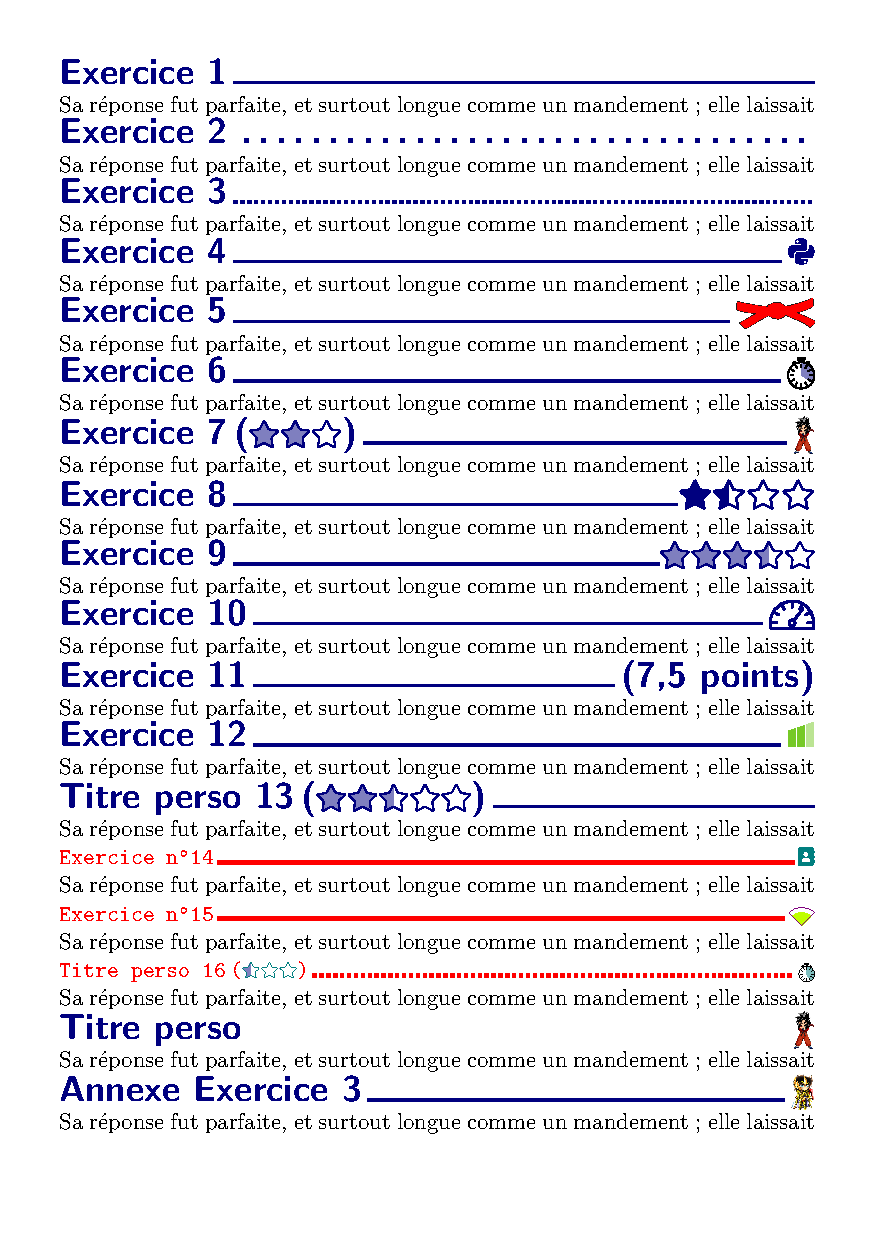
\includegraphics{envtexo_exemples.pdf}
\end{DemoCode}

\pagebreak

\section{Boîtes divers}

\subsection{Introduction}

L'idée est de proposer (modestement) des commandes, basées sur \MontreCode{tcolorbox}, pour, avec un style prédéfini :

\begin{itemize}
	\item créer des boîtes de présentation ;
	\item créer des titres de sujets d'examens, par exemple ;
	\item créer des titres d'exercices, pour des sujets d'examens par exemple ;
	\item créer des numéros encadrés ;
	\item créer de vignettes.
\end{itemize}

\subsection{Boîtes de présentation}

\begin{DemoCode}{listing only}
\begin{BoiteSimple}[couleur]<options tcbox>{titre}
	...
\end{BoiteSimple}
\end{DemoCode}

\begin{DemoCode}{}
\begin{BoiteSimple}[red]{Propriété}
Si M est la matrice d'adjacence d'un graphe simple orienté de sommets $A_1$, $A_2$, \dots, $A_n$, le nombre de chemins de longueur $p$ d'un sommet $A_i$  à un sommet $A_j$ est le nombre situé ligne $i$ et colonne $j$ dans la matrice $M^p$.
\end{BoiteSimple}
\end{DemoCode}

\begin{DemoCode}{}
\begin{BoiteSimple}[blue]<width=0.75\linewidth,flush right>{Propriété}
Si M est la matrice d'adjacence d'un graphe simple orienté de sommets $A_1$, $A_2$, \dots, $A_n$, le nombre de chemins de longueur $p$ d'un sommet $A_i$  à un sommet $A_j$ est le nombre situé ligne $i$ et colonne $j$ dans la matrice $M^p$.
\end{BoiteSimple}
\end{DemoCode}

\subsection{Titres de sujets d'examens, titres d'exercices}

\begin{DemoCode}{listing only}
\begin{TitreSujet}[Couleur=...,AlignH=...]<options tcbox>{titre onglet}
...
\end{TitreSujet}
\end{DemoCode}

\begin{DemoCode}{}
\begin{TitreSujet}[Couleur=red!50!black]{SUJET}
Métropole, SIO, 16 Mai 2024
\end{TitreSujet}
\end{DemoCode}

\begin{DemoCode}{}
\begin{TitreSujet}[Couleur=teal,AlignH=center]{CORRIGÉ}
Baccalauréat Centres étrangers Groupe 1\\
14 mars 2023
\end{TitreSujet}
\end{DemoCode}

\begin{DemoCode}{listing only}
\SujetTitreExo[couleur]{titre}
\end{DemoCode}

\begin{DemoCode}{}
\SujetTitreExo{Exercice 4 (5 points)}

\SujetTitreExo[olive]{Exercice 1 [Matrices]\dotfill(5 points)}
\end{DemoCode}

\subsection{Numéros encerclés}

\begin{DemoCode}{listing only}
\CircledNumber[bg=...,txt=...,bthick=...,bcol=...,raise=true/false]%
    {nombre}{noeud tikz}
\end{DemoCode}

\begin{DemoCode}{}
En ligne \CircledNumber{1} avec texte après.
\end{DemoCode}

\begin{DemoCode}{}
{\bfseries\sffamily\Huge En ligne (\CircledNumber[bthick=0.25mm,bcol=red,bg=cyan!25,txt=darkgray]{7}) avec texte après}
\end{DemoCode}

\begin{DemoCode}{}
{\Large En ligne \CircledNumber[raise=false,bthick=0.5mm,bcol=cyan,bg=cyan!25,txt=orange]{4} avec texte après}
\end{DemoCode}

\begin{DemoCode}{}
\begin{enumerate}[label={\CircledNumber[raise=false]{\arabic*}}]
	\item A
	\item B
	\item C
\end{enumerate}
\end{DemoCode}

\subsection{Vignettes}

\begin{DemoCode}{listing only}
\AffVignette(*)[Type=...,Couleur=...,Police=...]{texte}
% la version étoilée active le \NoAutoSpacing
\end{DemoCode}

\begin{DemoCode}{}
%vignette de base
\AffVignette{test} ou \AffVignette[Couleur=magenta]{test}
\end{DemoCode}

\begin{DemoCode}{}
%vignette type algo
\AffVignette[Type=algo]{test} ou \AffVignette[Type=algo,Couleur=teal]{Renvoyer}
\end{DemoCode}

\begin{DemoCode}{}
%vignette type python, classique
\AffVignette[Type=py]{test} ou \AffVignette[Type=py,Couleur=lime]{return}

%vignette type python, avec piton (et lualatex)
%\AffVignette[Type=pypit]{from math import sqrt}

%vignette type python, avec piton et pyluatex (et lualatex + shell-escape)
%\AffVignette[Type=pyl,Couleur=blue]{1+4/5}
\end{DemoCode}

\begin{DemoCode}{}
%vignette type graphique
\AffVignette[Type=grph]{fonction} ou \AffVignette[Couleur=olive,Type=grph]{intersection}
\end{DemoCode}

\begin{DemoCode}{}
%vignette type MPM
\AffVignette[Type=mpm]{marge} ou \AffVignette[Type=mpm,Couleur=orange]{chemin}
\end{DemoCode}

\begin{DemoCode}{}
%vignette type xcas
\AffVignette[Type=xcas]{calcul formel} ou \AffVignette[Type=xcas,Couleur=brown]{calcul formel}
\end{DemoCode}

\begin{DemoCode}{}
%vignette type shell
\AffVignette[Type=shell,Couleur=red!50!orange]{fenêtre cmd}
\end{DemoCode}

\begin{DemoCode}{}
%vignette type LaTeX
\AffVignette[Type=tex]{code LaTeX}
\end{DemoCode}

\begin{DemoCode}{}
%vignette type tableur
\AffVignette[Type=sheet,Couleur=green!50!black,Police=\footnotesize\sffamily]
    {cellule A3}
\end{DemoCode}

\begin{DemoCode}{}
%vignette type tableur
\AffVignette[Type=perso/CRYPT,Couleur=blue!50!teal,Echelle=0.5]
    {vignette personnalisée}
\end{DemoCode}

\begin{DemoCode}{}
%création d'une macro personnelle
\NewDocumentCommand\VignetteTableur{ m }{%
	\AffVignette*[Type=sheet,Couleur=green!50!black,Police=\footnotesize\sffamily]
	{#1}
}
On se place dans la plage \VignetteTableur{A3:B5} pour...

\end{DemoCode}

\subsection{Boîte arrondie, petite boîte type marker}

\begin{DemoCode}{listing only}
\BoiteArrondie[Fond=...,Texte=...,EspH=...,Style=...]{texte}[noeud tikz]
\end{DemoCode}

\begin{DemoCode}{}
On lance le logiciel \BoiteArrondie[Fond=cyan!33,Texte=violet,EspH=2mm,Style=rect]{situé sur le bureau} en cliquant \BoiteArrondie[Fond=lightgray!25,Texte=darkgray]{droit}.
\end{DemoCode}

\begin{DemoCode}{listing only}
\tbcmarker[Couleur=...,Largeur=...,Police=...]{contenu}
\end{DemoCode}

\begin{DemoCode}{}
\tbcmarker{contenu}
\end{DemoCode}

\begin{DemoCode}{}
\tbcmarker[Couleur=olive,Police=\normalfont\normalsize]{contenu}
\end{DemoCode}

%\subsection{Lettres à la manière d'un pixelart (expérimental)}
%
%L'idée est de proposer une présentation de (quelques) lettres (faite en \TikZ) sous la forme d'un \textit{pixelart}.
%
%\smallskip
%
%Par défaut les lettres ont une \textit{hauteur} de 5 carreaux (la taille est déterminée par rapport à la hauteur globale souhaitée, qui vaut par défaut 11~mm), et 2 carreaux ont été rajoutés en haut et en bas, et 1 carreau de chaque côté.
%
%\smallskip
%
%Attention cependant aux caractères spéciaux et/ ou aux lettres accentuées, qui pourraient poser problème (au quel cas la macro d'insertion individuelle est à préférer !)
%
%\begin{DemoCode}{listing only}
%%une lettre
%\PixlLetter%
%    [height=...,thick=...,color=...,gridcolor=...,
%    offseth=...,offsetv=...,gridafter=...,nospaceafter=...]
%    <options tikzpicture>
%    {lettre}
%
%%l'apostrophe, si besoin...
%\PixlLetterQuote%
%    [height=...,thick=...,color=...,gridcolor=...,
%    offseth=...,offsetv=...,gridafter=...,nospaceafter=...]
%    <options tikzpicture>
%
%%plusieurs lettres
%\PixlLetters%
%    [height=...,thick=...,color=...,gridcolor=...,
%    offseth=...,offsetv=...,gridafter=...,nospaceafter=...]
%    {lettres}
%\end{DemoCode}
%
%\begin{DemoCode}{listing only}
%\PixlLetter{S}\PixlLetter{i}\PixlLetter{n}\PixlLetter{g}\PixlLetter{e}
%
%\PixlLetters[height=2cm,color=red,gridafter,offsetv=1]{(Singe)}
%
%\PixlLetters[color=blue]{Les singes, c'est super !?}
%
%\PixlLetters[color=red]{1+1=2}
%\end{DemoCode}
%
%\PixlLetter{S}\PixlLetter{i}\PixlLetter{n}\PixlLetter{g}\PixlLetter{e}
%
%\PixlLetters[height=2cm,color=red,gridafter,offsetv=1]{(Singe)}
%
%\PixlLetters[color=blue]{Les singes, c'est super !?}
%
%\PixlLetters[color=red]{1+1=2}

\subsection{Bannière de titre}

L'idée est de proposer une bannière, réalisée en \TikZ, pour présenter par exemple un titre.

Il sera ensuite possible de redéfinir un sectionnement du document (\MontreCode{part/section/subsection/...}).

Le style global est fixé, mais des éléments de personnalisations sont possibles (des calculs en interne sont effectués pour adapter la taille des textes).

\begin{DemoCode}{listing only}
\tkzBannerTri[clés]{numéro}{titre}
\end{DemoCode}

\begin{DemoCode}{}
\tkzBannerTri{01}{Titre du document}
\end{DemoCode}

Les principales \MontreCode{clés} (anglicisées) sont :

\begin{itemize}
	\item \MontreCode{height} : hauteur de la bannière (\MontreCode{2.5em} par défaut)
	\item \MontreCode{width} : largeur de la bannière (\MontreCode{\textbackslash linewidth} par défaut)
	\item \MontreCode{blockwidth} : largeur du bloc gauche (\MontreCode{2.75em} par défaut, mais si \MontreCode{auto}, la largeur s'adaptera à son contenu)
	\item \MontreCode{coltxt} : couleur des textes (\MontreCode{white} par défaut)
	\item \MontreCode{fonttxt} : police globale des textes (\MontreCode{white} par défaut)
	\item \MontreCode{swap} : booléen pour changer le style de la partie droite (\MontreCode{false} par défaut)
	\item \MontreCode{maincolor} : couleur principale, les dégradés étant calculés automatiquement (\MontreCode{darkgray} par défaut)
	\item \MontreCode{collight} : couleur la plus claire (\MontreCode{darkgray!25} par défaut)
	\item \MontreCode{colmedium} : couleur du milieu (\MontreCode{darkgray!50} par défaut)
	\item \MontreCode{coldark} : couleur la plus foncée (\MontreCode{darkgray} par défaut)
	\item \MontreCode{logo} : logo éventuel, placé tout à droite
	\item \MontreCode{type} : type éventuel du document, qui est dans le bloc gauche
	\item \MontreCode{dispblock} : booléen pour afficher le bloc de gauche (actif par défaut)
	\item \MontreCode{num} : booléen pour afficher le numéro (actif par défaut)
	\item \MontreCode{customtype} : texte personnalisé éventuel du bloc gauche
	\item \MontreCode{custommulti} : booléen pour un texte personnalisé éventuel du bloc gauche sur deux lignes
\end{itemize}

\begin{DemoCode}{}
\tkzBannerTri
	[maincolor=red,type=EXERCICES,blockwidth=auto,logo=\faAddressBook]
	{7}{Mon document}
\end{DemoCode}

\begin{DemoCode}{}
\tkzBannerTri
	[maincolor=red,type=EXERCICES,blockwidth=5em,logo=\faAddressBook]
	{7}{Mon document}
\end{DemoCode}

\begin{DemoCode}{}
\tkzBannerTri[%
	maincolor=red,type=EXERCICES,blockwidth=auto,logo=\faAddressBook,swap]
	{07}{Mon document}
\end{DemoCode}

\begin{DemoCode}{}
\tkzBannerTri
	[dispblock=false,maincolor=teal,logo=\faSchool]
	{}{Mon document}
\end{DemoCode}

\begin{DemoCode}{}
\tkzBannerTri
	[maincolor=olive,customtype=TP,blockwidth=4em,logo=\faAddressBook,height=4em]
	{7}{Mon document}
\end{DemoCode}

Il est de ce fait \textit{normalement} possible (à vérifier quand même avec une insertion dans une \textsf{toc}\ldots) de modifier le comportement de la commande \MontreCode{\textbackslash part}, dans l'optique de l'utilisation avec une table des matières notamment.

%\begin{DemoCode}{}
%%redéfinition de \part avec gestion de la version étoilée
%\RenewDocumentCommand\part{ s m D<>{} }{%
%	\addtocounter{part}{1}%
%	\IfBooleanTF{#1}%
%		{%
%			\tkzBannerTri[#3,num=false]{\thepart}{#2}%
%		}%
%		{%
%			\tkzBannerTri[#3]{\thepart}{#2}%
%			%\addcontentsline{toc}{part}{#2}%éventuellement
%		}%
%}
%%modification de la numérotation, avec forçage du 0
%\renewcommand\thepart{\ifnum\value{part}<10\relax0\fi\arabic{part}}
%
%\part{Éléments de logique}<type=TP,logo=\faAirbnb>
%\end{DemoCode}

\pagebreak

À noter qu'il existe une commande \textit{alternative}, avec un fonctionnement légèrement différent, puisque la hauteur de la bannière et la largeur du bloc sont fixés, de sorte que les labels s'adaptent automatiquement.

Les \MontreCode{clés} sont les mêmes, le fonctionnement global également, à l'exception de la clé \MontreCode{[customtype]} en mode \MontreCode{custommulti} qui doit être donné sous la forme \MontreCode{[customtype=L1+L2]}.

\begin{DemoCode}{}
\tkzBannerTriAlt
	[maincolor=magenta,logo=\faSchool,type=INTERRO]
	{05}{Mon document}

\tkzBannerTriAlt
	[maincolor=violet,swap,logo=\faSchool,customtype={INTERRO+DE COURS},custommulti,blockwidth=1.25cm]
	{}{Probabilités (v1)}
\end{DemoCode}

\pagebreak

\subsection{Panneaux autoroutiers}

L'idée est de proposer des panneaux type \textit{autoroutes}, réalisés via \MontreCode{tcolorbox}.

Le style global est fixé, mais des éléments de personnalisations sont possibles..

\begin{DemoCode}{listing only}
\begin{PanneauAutoroute}[clés]{titre}
%contenu
\end{PanneauAutoroute}
\end{DemoCode}

\begin{DemoCode}{}
\begin{PanneauAutoroute}{A4}
REIMS\hfill~145\\
PARIS\hfill~250
\end{PanneauAutoroute}
\end{DemoCode}

Les clés, optionnelles et entre \MontreCode{[...]} sont :

\begin{itemize}
	\item \MontreCode{Fleches} : nombre de flèches à afficher (\MontreCode{0} par défaut)
	\item \MontreCode{CouleurFond} : couleur de fond (\MontreCode{blue} par défaut)
	\item \MontreCode{CouleurTitre} : couleur de la boîte \textit{titre} (\MontreCode{red} par défaut)
	\item \MontreCode{Largeur} : largeur du panneau (\MontreCode{10cm} par défaut)
	\item \MontreCode{Police} : police du panneau
	\item \MontreCode{PoliceCartouche} : police du titre
	\item \MontreCode{TypeFleche} : flèche(s) à afficher
	\item \MontreCode{EspacementV} : interligne (\MontreCode{2.5mm} par défaut)
	\item \MontreCode{Dernier} : booléen pour préciser que la boîte sera la dernière de la série (pour l'espace après).
\end{itemize}

\begin{DemoCode}{}
\begin{PanneauAutoroute}[Largeur=\linewidth,Dernier=false]{TD01}
	\VilleDist{COMPETENCE 1}{\faCheck}  %macro interne pour afficher une ligne
	\VilleDist*{COMPETENCE 2}{\faCheck} %macro pour afficher la dernière ligne
\end{PanneauAutoroute}

\begin{PanneauAutoroute}%
	[CouleurFond=olive,Fleches=2,Police=\bfseries\huge\fontfamily{phv}\selectfont]{}
	LILLE\hfill~301\\
	AMIENS\hfill~213
\end{PanneauAutoroute}
\end{DemoCode}

\pagebreak

\subsection{Affichettes de soldes}

L'idée est de proposer des petites affichettes pour des réductions, réalisées via \MontreCode{tcolorbox} (sur une idée de \textit{Sébastien Lozano}).

Le style global est fixé, mais des éléments de personnalisations sont possibles..

\begin{DemoCode}{listing only}
\AfficheSoldes[clés]{prix avant}{prix après}{réduction}
\end{DemoCode}

\begin{DemoCode}{}
\AfficheSoldes{99\texteuro}{79\texteuro}{-20\%}
\end{DemoCode}

Les clés, optionnelles et entre \MontreCode{[...]} sont :

\begin{itemize}
	\item \MontreCode{Couleur} : couleur principale (\MontreCode{gray} par défaut)
	\item \MontreCode{Largeur} : largeur (\MontreCode{auto} ou par défaut) à définir
	\item \MontreCode{PoliceEntete} : police du titre
	\item \MontreCode{PolicePrix} : police des prix
	\item \MontreCode{PoliceReduc} : police de la réduction
	\item \MontreCode{Titre} : titre de l'affiche (\MontreCode{GRANDE DÉMARQUE} par défaut)
	\item \MontreCode{OffsetReduc} : \textit{pente} pour le bandeau de réduction (\MontreCode{1.25cm} par défaut)
	\item \MontreCode{AgrandirReduc} : augmenter la hauteur de la partie réduction
\end{itemize}

Donc la hauteur est fixée par \textit{calculs}, et également la largeur si \MontreCode{Largeur=auto}.

La largeur \MontreCode{auto} permet de faire \textit{marcher} des prix jusque \MontreCode{99\,999\,€}.

\begin{DemoCode}{}
\AfficheSoldes{99\texteuro}{79\texteuro}{-20\,\%}~%
\AfficheSoldes[Couleur=red]{99\texteuro}{79\texteuro}{-20\,\%}~%
\AfficheSoldes[Couleur=blue]{\ldots\texteuro}{79\texteuro}{-20\,\%}~%
\AfficheSoldes[Couleur=teal]{\ldots}{\ldots}{\ldots}
\end{DemoCode}

\begin{DemoCode}{}
\AfficheSoldes[%
		Couleur=magenta,%
		Largeur=6cm,%
		PoliceEntete=\huge\sffamily\bfseries,%
		PolicePrix=\ttfamily,%
		PoliceReduc=\bfseries\Huge\sffamily,%
		AgrandirReduc=8mm
		]%
	{1\,500\texteuro}{1\,299\texteuro}{-\ldots\,\%}
\end{DemoCode}

\begin{DemoCode}{}
\AfficheSoldes[%
		Couleur=cyan,%
		PoliceEntete=\bfseries\huge\fontfamily{qhv}\selectfont,%
		PolicePrix=\fontfamily{qhv}\selectfont,%
		PoliceReduc=\bfseries\Huge\fontfamily{qhv}\selectfont,%
		AgrandirReduc=1cm
		]%
	{\makebox[1cm]{\dotfill}\texteuro}{1\,299\texteuro}{-30\,\%}
\end{DemoCode}

\pagebreak

\section{Patchs divers}

\subsection{Gérer l'espacement vertical du mode hors-ligne}

L'idée est de proposer une commande, à insérer dans le préambule, pour \textit{patcher} l'espacement vertical proposé par les environnements mathématiques hors-ligne.

\begin{DemoCode}{listing only}
...
\ChangerDisplaySkip[clés]
...
\begin{document}
\end{DemoCode}

Les \MontreCode{clés} disponibles, à donner entre \MontreCode{[...]}, sont :

\begin{itemize}
	\item \MontreCode{Avant=...} : modification de l'espacement avant ;
	\item \MontreCode{AvantS=...} : modification de l'espacement avant (version \textit{short}) ;
	\item \MontreCode{Apres=...} : modification de l'espacement après ;
	\item \MontreCode{ApresS=...} : modification de l'espacement après (version \textit{short}) ;
	\item \MontreCode{Global=...} : modification globale de \textbf{tous} les espacements ;
	\item \MontreCode{Dense} : booléen pour modification globale en \MontreCode{0.33\textbackslash baselineskip}.
\end{itemize}

\subsection{Quelques ajouts au package pas-tableur}

L'idée est de proposer quelques commandes complémentaires pour le package \textsf{pas-tableur}, de Stéphane Pasquet (\url{https://ctan.org/pkg/pas-tableur}), en respectant autant que faire se peut la syntaxe du package (voir la documentation pour de plus amples informations).

\smallskip

Le package \textsf{pas-tableur} n'est pas chargé par défaut, mais il peut l'être grâce à l'option \MontreCode{[pastableur]}.

\smallskip

Les \textit{ajouts} disponibles sont :

\begin{itemize}
	\item colorer/griser une case, via \MontreCode{\textbackslash celcouleur} ;
	\item fusionner des celules, via \MontreCode{\textbackslash celfusion} ;
	\item \textit{casser la numérotation} avec des pointillés, via \MontreCode{\textbackslash celnumbreak} ;
	\item remplir (partiellement ou non) une ligne,  via \MontreCode{\textbackslash lignetxt} ;
	\item remplir (partiellement ou non) une colonne,  via \MontreCode{\textbackslash colonnetxt}.
\end{itemize}

\begin{DemoCode}{listing only}
%chargement du package
\usepackage[pastableur]{customenvs}

%griser une cellule
\celcouleur[couleur]{col-lig}

%fusionner des cellules
\celfusion[options pas-tableur]{col-lig}{col-lig}{label}

%pointillés dans la numérotation
\celnumbreak{num ligne pointillés}{début numéro suite}{fin numéro suite}

%remplir ligne
\lignetxt(*)[options pas-tableur]{num ligne}<col début>{liste des cellules}

%remplir colonne
\colonnetxt(*)[options pas-tableur]{num colonne}<lgn début>{liste des cellules}
\end{DemoCode}

\pagebreak

L'exemple suivant illustre les différentes commandes proposées dans ce package.

\begin{DemoCode}{}
\begin{tikzpicture}{}
	\tableur*[10]{A/2.5cm,B/2.5cm,C/2.5cm,D/2.5cm,E/2.5cm,F/2.5cm}
	%ligne n°1
	\celtxt*[align=center]{A}{1}{$n$}
	\celfusion[align=center]{B-1}{C-1}{$M_n$}
	\celfusion[align=center]{D-1}{E-1}{$S_n$}
	\celtxt*[align=center]{F}{1}{$d_n$}
	%		%Ligne2/3/4
	\celcouleur{A-2}
	\lignetxt*[align=center]{2}<2>{$x_n$,$y_n$,5,$n$,$n$} %à partir de la colonne n°2
	\lignetxt*[align=center]{3}{0,0,0,5,0,5}
	\lignetxt*[align=center]{4}{1,1,0,5,1,4.12310563}%
	\celnumbreak{8}{27}{28}
	%colonneA
	\colonnetxt*[align=center]{A}<5>{2,3,4,\dots,24,25}   %à partir de la ligne n°5
\end{tikzpicture}
\end{DemoCode}

\subsection{Insertion d'images avec remplissage de l'espace vertical}

L'idée est de proposer une commande pour adapter la hauteur d'une image à la hauteur restante en base de page.

Cela repose en fait simplement sur l'utilisation de \MontreCode{[height=\textbackslash dimexpr\textbackslash pagegoal-\textbackslash pagetotal\textbackslash relax]}.

\begin{DemoCode}{listing only}
\InsererImage<vRemplir=true/false,vOffset=...,vCentrer=...>[clés includegraphics]<image>
\end{DemoCode}

La clé \MontreCode{vOffset} permet de spécifier une longueur à retirer au calcul automatique (par défaut elle est fixée à \MontreCode{0pt})..

La clé \MontreCode{vCentrer} (parmi \MontreCode{m/h/b/n} permet de spécifier un type de centrage vertical, si besoin, parmi \MontreCode{milieu/haut/bas/non} (\MontreCode{n} par défaut).

\begin{DemoCode}{listing only}
\InsererImage<vRemplir,vOffset=5mm,vCentrer=m>{example-image}
\end{DemoCode}

\InsererImage<vRemplir,vOffset=5mm,vCentrer=m>{example-image}

\subsection{Grille automatique pour les environnements tikzpicture}

L'idée est de proposer de quoi afficher, en \textit{surimpression}, une grille automatique sur une figure \MontreCode{tikzpicture}.

Cela peut-être utile dans la construction de graphes ou de figures géométriques pour placer plus facilement des objets.

\smallskip

Il est possible de :

\begin{itemize}
	\item demander ponctuellement l'affichage avec une macro à placer en fin d'environnement ;
	\item automatiser l'affichage pour une figure avec une \MontreCode{clé} et une macro locale ;
	\item automatiser l'affichage pour toutes les figures avec une macro globale et une \MontreCode{clé}.
\end{itemize}

\textbf{\large Version manuelle}

\begin{DemoCode}{listing only}
%macro locale, utilisation ponctuelle
\begin{tikzpicture}
	%codes
	\tkzGrilleAuto(*){pasX§pasY}
\end{tikzpicture}
\end{DemoCode}

La version étoilée marque également l'origine $(0;0)$.

L'argument obligatoire permet de spécifier les pas (\texttt{H§V}) pour la grille.

\begin{DemoCode}{}
\begin{tikzpicture}
	%population
	\draw[very thick,purple] (0,0) circle[x radius=3cm,y radius=2cm] ;
	\draw[purple] (0.5,1.25) node[font=\small] {Population E} ;
	%ss population
	\draw[very thick,teal] (-0.75,-0.25) circle[x radius=1.75cm,y radius=1cm] ;
	\draw[teal] (-0.75,-0.25) node[font=\small] {Sous-population A} ;
	%grille auto manuelle, avec origine
	\tkzGrilleAuto*{0.5§0.5}
\end{tikzpicture}
\end{DemoCode}

\textbf{\large Version automatique locale, avec clé}

\begin{DemoCode}{listing only}
%clé locale, utilisation ponctuelle
\begin{tikzpicture}[grilleauto=pasX§pasY]
	\tkzAutoGridLocal(*)
	%codes
\end{tikzpicture}
\end{DemoCode}

La version étoilée marque également l'origine $(0;0)$.

\begin{DemoCode}{}
\begin{tikzpicture}[x=0.5cm,y=0.5cm,grilleauto=0.25§0.25]
	%grille (qui sera affichée en dernier)
	\tkzAutoGridLocal*
	%triangle
	\draw[very thick,red] (-4,-2)--(0,7)--(6,1)--cycle ;
	%cercle
	\draw[very thick,blue] (0,0) circle[radius=5] ;
	%segment
	\draw[very thick,orange] (-1.75,1.25)--(1,-7);
\end{tikzpicture}
\end{DemoCode}

\textbf{\large Version automatique globale, avec clé}

\begin{DemoCode}{listing only}
%préambule, la commande sera active pour tous les environnements tikz
\tkzAutoGridActivate(*)

%document
\begin{tikzpicture}[grilleauto=pasX§pasY]
	%codes
\end{tikzpicture}
\end{DemoCode}

La version étoilée marquera également l'origine $(0;0)$.

\pagebreak

\subsection{Flèche évasée, en \TikZ}

L'idée est de proposer une commande, en  \TikZ, pour représenter une flèche évasée, avec des paramètres optionnels.

\begin{DemoCode}{listing only}
\tkzFlecheEvasee[clés]{départ}{arrivée ou déplacement}
\end{DemoCode}

\begin{DemoCode}{}
\begin{tikzpicture}
	\tkzFlecheEvasee{0,0}{5,1.5}
\end{tikzpicture}
\end{DemoCode}

Les \MontreCode{clés} disponibles, à donner entre \MontreCode{[...]}, sont :

\begin{itemize}
	\item \MontreCode{Couleur=...} : couleur de la flèche ;
	\item \MontreCode{Epaisseur=...} : taille initiale du trait (\MontreCode{0.5mm} par défaut) ;
	\item \MontreCode{Direction=...} : direction de la flèche, avec angle éventuel ;
	\item \MontreCode{Coeff=...} : coefficient pour la taille finale du trait (\MontreCode{4} par défaut) ;
	\item \MontreCode{TypeFleche=...} : type de la flèche, issue de \MontreCode{arrows.meta} ;
	\item \MontreCode{TailleFleche=...} : booléen pour la taille de la partie flèche (\MontreCode{auto} par défaut), en langage \MontreCode{arrows.meta} ;
	\item \MontreCode{Deplacement} : booléen pour spécifier qu'on travaille avec un déplacement pour l'arrivée.
\end{itemize}

Le premier argument obligatoire, permet de spécifier le nœud de départ ou les coordonnées du point de départ.

Le second argument obligatoire, permet de spécifier le nœud d'arrivée ou les coordonnées du point d'arrivée, mais également le déplacement dans le cas ou \MontreCode{Deplacement=true}.

\medskip

Par défaut, et en mode \MontreCode{auto} :

\begin{itemize}
	\item le début du trait mesure \MontreCode{Epaisseur=0.5mm} ;
	\item la fin du trait mesure \MontreCode{4*Epaisseur=2mm} ;
	\item les dimensions de la flèche sont \MontreCode{H=2*4*Epaisseur=4mm} et \MontreCode{L=2.1*4*Epaisseur=4.2mm}.
\end{itemize}

À noter que pour les flèches type \MontreCode{Stealth}, un ajustement est sans doute à prévoir pour compenser le \textit{creux}.

\begin{DemoCode}{}
%flèche 0.5mm -> 1.25mm
\begin{tikzpicture}
	\tkzFlecheEvasee%
		[Epaisseur=0.5mm,Coeff=2.5,Direction=left/30,Couleur=red,TypeFleche=Triangle]%
		{0,0}{5,1.5}
\end{tikzpicture}
\end{DemoCode}

\begin{DemoCode}{}
\begin{tikzpicture}
	\draw[thin,lightgray] (-3,-1) grid (5,5) ;
	\coordinate (A) at (0,0) ; \coordinate (B) at (4,1) ;
	\coordinate (C) at (1,1) ; \coordinate (D) at (5,4) ;
	\coordinate (E) at (0,1) ; \coordinate (F) at (0,5) ;
	\coordinate (G) at (-2,0) ;
	\tkzFlecheEvasee[Couleur=green,TypeFleche=Triangle]{A}{B}
	\tkzFlecheEvasee[Couleur=blue,Direction=right/10]{D}{C}
	\tkzFlecheEvasee%
		[Couleur=red,Direction=left/45,TypeFleche=Stealth,Epaisseur=0.1mm,Coeff=10]%
		{-2,1}{0,4}
	\tkzFlecheEvasee%
		[Couleur=red,Direction=right/45,Epaisseur=0.1mm,Coeff=10,TypeFleche=Stealth]%
		{-2,1}{0,4}
	\tkzFlecheEvasee[Couleur=teal,Deplacement,Direction=left/10]{-3,-1}{5,1}
\end{tikzpicture}
\end{DemoCode}

\pagebreak

\subsection{Annoter une image}

L'idée est de proposer de quoi annoter une image, en utilisant un environnement et une commande qui sont liés à \TikZ.

\begin{DemoCode}{listing only}
\begin{AnnoterImage}[clés][options includegraphics]{image}
	\PlacerTxtSurImg[options node tikz]{coordonnées}{texte}
	\PlacerTxtSurImg*[options node tikz]{coordonnées en pourcentage}{texte}
	%code tikz
\end{AnnoterImage}
\end{DemoCode}

\begin{DemoCode}{}
%\usepackage[auto,outline]{contour}
\begin{AnnoterImage}[Grille=0.5][height=4cm]{example-image.png}
	\PlacerTxtSurImg[scale=5,rotate=30]
		{1,1}{\contourlength{0.05em}\color{white}\contour{black}{$\pi$}}
	\PlacerTxtSurImg*[scale=1.5,rotate=-15]
		{0.66,0.75}{\contourlength{0.025em}\color{violet}\contour{yellow}{Pythagore}}
\end{AnnoterImage}
\end{DemoCode}

Concernant l'environnement, les \MontreCode{clés} disponibles (premier argument), à donner entre \MontreCode{[...]}, sont :

\begin{itemize}
	\item \MontreCode{Noeud=...} : nom du nœud créé (si réutilisation avec un \texttt{remember picture}) ;
	\item \MontreCode{Grille=...} : Grille éventuelle d'aide (en unité) (\MontreCode{vide} par défaut) ;
	\item \MontreCode{SousGrille=...} : sous-grille éventuelle (\MontreCode{4} par défaut) ;
	\item \MontreCode{CouleurGrille=...} : couleur de la grille d'aide (\MontreCode{teal} par défaut) ;
	\item \MontreCode{Clip=...} : booléen pour fixer les annotations à l'intérieur de l'image (\MontreCode{true}).
\end{itemize}

Le deuxième argument, optionnel et entre \MontreCode{[...]}, correspond aux options spécifiques liées à \MontreCode{includegraphics}.

Le fichier est à préciser avec sont extension, car le code se charge de vérifier que le fichier existe.

\begin{DemoCode}{}
\begin{AnnoterImage}[Noeud=TESTIMG][height=3.75cm]<rotate=15>{example-image-golden.pdf}
	%commandes manuelles
	\draw (TESTIMG.center) node[above=5mm,font=\Huge\ttfamily\bfseries,text=blue] {TEST1} ;
	\draw (TESTIMG.north west) node[draw,thick,red,inner sep=0.5mm,below right=2.5mm,font=\LARGE\sffamily\bfseries,text=red] {TEST2} ;
\end{AnnoterImage}
\end{DemoCode}

\pagebreak

\subsection{Travailler sur des longueurs}

L'idée est de proposer de quoi déterminer la plus grande largeur d'une liste de textes. Il est ainsi possible (même si le but des polices à chasses non fixes n'est pas celui-là\ldots) d'\textit{aligner} verticalement des textes de présentation par exemple.

\begin{DemoCode}{listing only}
\getwideststring[macro de stockage]{elt1,elt2,...eltn}

\halignmakebox[alig option]{elt}{list of elements}
\end{DemoCode}

\begin{DemoCode}{}
%récupération de la plus grande largeur (\tmpwideststring par défaut)
\getwideststring{Exercice 1,Évaluation 2,Test n°3}\the\tmpwideststring
\end{DemoCode}

\begin{DemoCode}{}
\sffamily\Large
Exercice 1 (10 points)\\
Évaluation 2 (8 points) \\
Test n°3 (4 points)
\end{DemoCode}

\begin{DemoCode}{}
%avec alignement
\sffamily\Large
\halignmakebox[l]{Exercice 1}{Exercice 1,Évaluation 2,Test n°3} 
(\halignmakebox[r]{10}{10,8,4} points)

\halignmakebox[l]{Évaluation 2}{Exercice 1,Évaluation 2,Test n°3} 
(\halignmakebox[r]{8}{10,8,4} points)

\halignmakebox[l]{Test n°3}{Exercice 1,Évaluation 2,Test n°3} 
(\halignmakebox[r]{4}{10,8,4} points)
\end{DemoCode}

À noter que des commandes sont disponibles pour stocker des dimensions d'une \textit{boîte} dans une macro (existante ou non) et éventuellement lui rajouter une valeur.

\begin{DemoCode}{listing only}
%largeur
\storewidthtolength[delta]{box}{\macro}
%hauteur
\storeheighttolength[delta]{box}{\macro}
%hauteur totale
\storetotalheighttolength[delta]{box}{\macro}
%profondeur
\storedepthtolength[delta]{box}{\macro}
\end{DemoCode}

\begin{DemoCode}{}
\def\tmpbox{\large $1+\frac{1}{x}$}
%
\storewidthtolength{\tmpbox}{\mytmpboxwidth}\the\mytmpboxwidth

\storewidthtolength[10pt]{\tmpbox}{\mytmpboxwidthdelta}\the\mytmpboxwidthdelta

\storeheighttolength{\tmpbox}{\mytmpboxheight}\the\mytmpboxheight

\storetotalheighttolength{\tmpbox}{\mytmpboxtotheight}\the\mytmpboxtotheight

\storedepthtolength{\tmpbox}{\mytmpboxdepth}\the\mytmpboxdepth
\end{DemoCode}

\begin{center}
	\def\tmpbox{\large $1+\frac{1}{x}$}%
	\storewidthtolength{\tmpbox}{\mytmpboxwidth}%
	\storeheighttolength{\tmpbox}{\mytmpboxheight}%
	\storetotalheighttolength{\tmpbox}{\mytmpboxtotheight}%
	\storedepthtolength{\tmpbox}{\mytmpboxdepth}%
	\begin{tikzpicture}[scale=5,transform shape]
		\node[draw=lightgray,inner sep=0pt,text=black] (BOX) {\large $1+\frac{1}{x}$} ;
		\begin{scope}
			\clip (BOX) ;
			\draw[lightgray] ([yshift=\mytmpboxdepth]BOX.south west) --++ ({\mytmpboxwidth+2\pgflinewidth},0) ;
		\end{scope}
		\draw[lightgray] ([yshift=\mytmpboxdepth]BOX.south west) --++ ({\mytmpboxwidth},0) ;
		\draw[<->,>=latex] ([yshift=-2pt]BOX.south west) --++ ({\mytmpboxwidth},0) node[midway,below,scale=0.2] {\the\mytmpboxwidth} ;
		\draw[<->,>=latex] ([xshift=-2pt]BOX.south west) --++ (0,\mytmpboxdepth) node[midway,left,scale=0.2] {\the\mytmpboxdepth} ;
		\draw[<->,>=latex] ([xshift=-2pt]BOX.north west) --++ (0,-\mytmpboxheight) node[midway,left,scale=0.2] {\the\mytmpboxheight} ;
		\draw[<->,>=latex] ([xshift=2pt]BOX.south east) --++ (0,\mytmpboxtotheight) node[midway,right,scale=0.2] {\the\mytmpboxtotheight} ;
	\end{tikzpicture}
\end{center}

\end{document}